\newpage
~
\newpage
\section{Propuesta}
Ya que es un tfg de desarrollo describimos lo realizado y cómo, así como los resultados obtenidos.

Una vez analizado el estado del arte y las tecnologías disponibles, se ha definido una propuesta de desarrollo que busca cumplir con los objetivos planteados en la introducción. Esta propuesta se basa en el uso de metodologías ágiles y tecnologías modernas para garantizar un desarrollo eficiente y escalable.

Tal como se ha especificado en el apartado anterior, se desarrollará una solución que busca ofrecer:
\begin{itemize}
    \item Solución FOSS que permita una aportar al proyecto de manera sencilla, pudiendo entender rápida y fácilmente el código y la arquitectura del sistema.
    \item Soluciones eficientes y rápidas. Para ello usaremos tecnologías lo más eficientes posibles, siempre buscando la seguridad y escalabilidad de la aplicación.
    \item Solución escalable y mantenible. Se busca que la solución sea escalable y mantenible a largo plazo, permitiendo añadir nuevas funcionalidades y mejoras de manera sencilla. Para ello se implementará una arquitectura limpia \parencite{uncle-bob-clean-architecture}, lo que nos proporcionará una estructura del proyecto completamente desacoplada, facilitando la escalabilidad y mantenimiento.
    \item Almacenamiento eficiente. Se busca que el almacenamiento de los archivos sea lo más eficiente posible, tanto en términos de espacio como de velocidad de acceso.
        Para ello, primero se hará uso de un sistema de almacenamiento de objetos compatible con S3, lo que nos permitirá utilizar cualquier servicio de almacenamiento compatible con S3 como Amazon S3, Google Cloud Storage y en nuestro caso, MinIO.
        Más adelante, se implementará una solución de almacenamiento nativa que permita un acceso más rápido y eficiente a los archivos, además de una mejor gestión de los mismos.
    \item Desarrollo ágil y flexible. Se busca que el desarrollo sea ágil y flexible, permitiendo adaptarse a los cambios y necesidades del proyecto de manera rápida y eficiente. Para ello se hará uso de la metodología ágil Scrum, lo que nos permitirá tener una organización clara del proyecto y una planificación adecuada de las tareas a realizar.
        Seguir esta metodología nos ayudará a tener una mejor organización del proyecto y una planificación adecuada de las tareas a realizar, lo que aportará una buena organización en un futuro si se incorporan más personas al proyecto.
\end{itemize}

\subsection{Metodología}
\label{sec:metodologia}

Para el desarrollo de este proyecto se va a hacer uso de la metodología ágil Scrum. Esta metodología se basa en el desarrollo iterativo e incremental, lo que permite una mayor flexibilidad y adaptación a los cambios durante el proceso de desarrollo.

Se ha optado por el uso de Scrum en vez de otra metodología ágil como Kanban o XP (Extreme Programming) o alguna metodología tradicional ya que se ha utilizado anteriormente y se considera que es con la que más cómodo y eficaz se va trabajar.

Tal y como se explica en la guía oficial de Scrum \parencite{scrum-guide}, Scrum es un marco de trabajo ágil que se utiliza para gestionar proyectos complejos y adaptarse a los cambios de manera rápida y eficiente. Se basa en la colaboración entre equipos multidisciplinarios, la entrega continua de valor y la mejora continua.
Scrum se centra en la entrega de incrementos de producto funcionales en ciclos cortos, lo que permite a los equipos recibir retroalimentación temprana y ajustar su enfoque según sea necesario. Esto es especialmente útil en proyectos donde los requisitos pueden cambiar con frecuencia o donde la incertidumbre es alta.

Scrum se basa en una serie de roles, eventos y artefactos que ayudan a los equipos a organizar su trabajo y colaborar de manera efectiva. Los roles incluyen el Product Owner (responsable de la visión del producto), el Scrum Master (facilitador del proceso) y el equipo de desarrollo (responsable de la entrega del producto). Los eventos incluyen las reuniones diarias, las revisiones de sprint y las retrospectivas, que permiten a los equipos reflexionar sobre su trabajo y mejorar continuamente.

Aunque Scrum está muy enfocado a equipos, también es posible utilizarlo con un equipo muy pequeño o incluso con una sola persona, realizando los mismos eventos pero sin la necesidad de tener un equipo de desarrollo.
Éste es el enfoque que se le va a dar a este proyecto. Una buena práctica de Scrum es documentar todas las reuniones y tomas de decisiones que se toman a lo largo de la vida del proyecto, ya que esto ayuda a tener una mejor organización y a poder ver cómo ha ido evolucionando el proyecto a lo largo del tiempo.
Es por ello que se van a documentar todas las decisiones que se tomen y los cambios que se realicen en el desarrollo.


\begin{figure}[H]
  \centering
  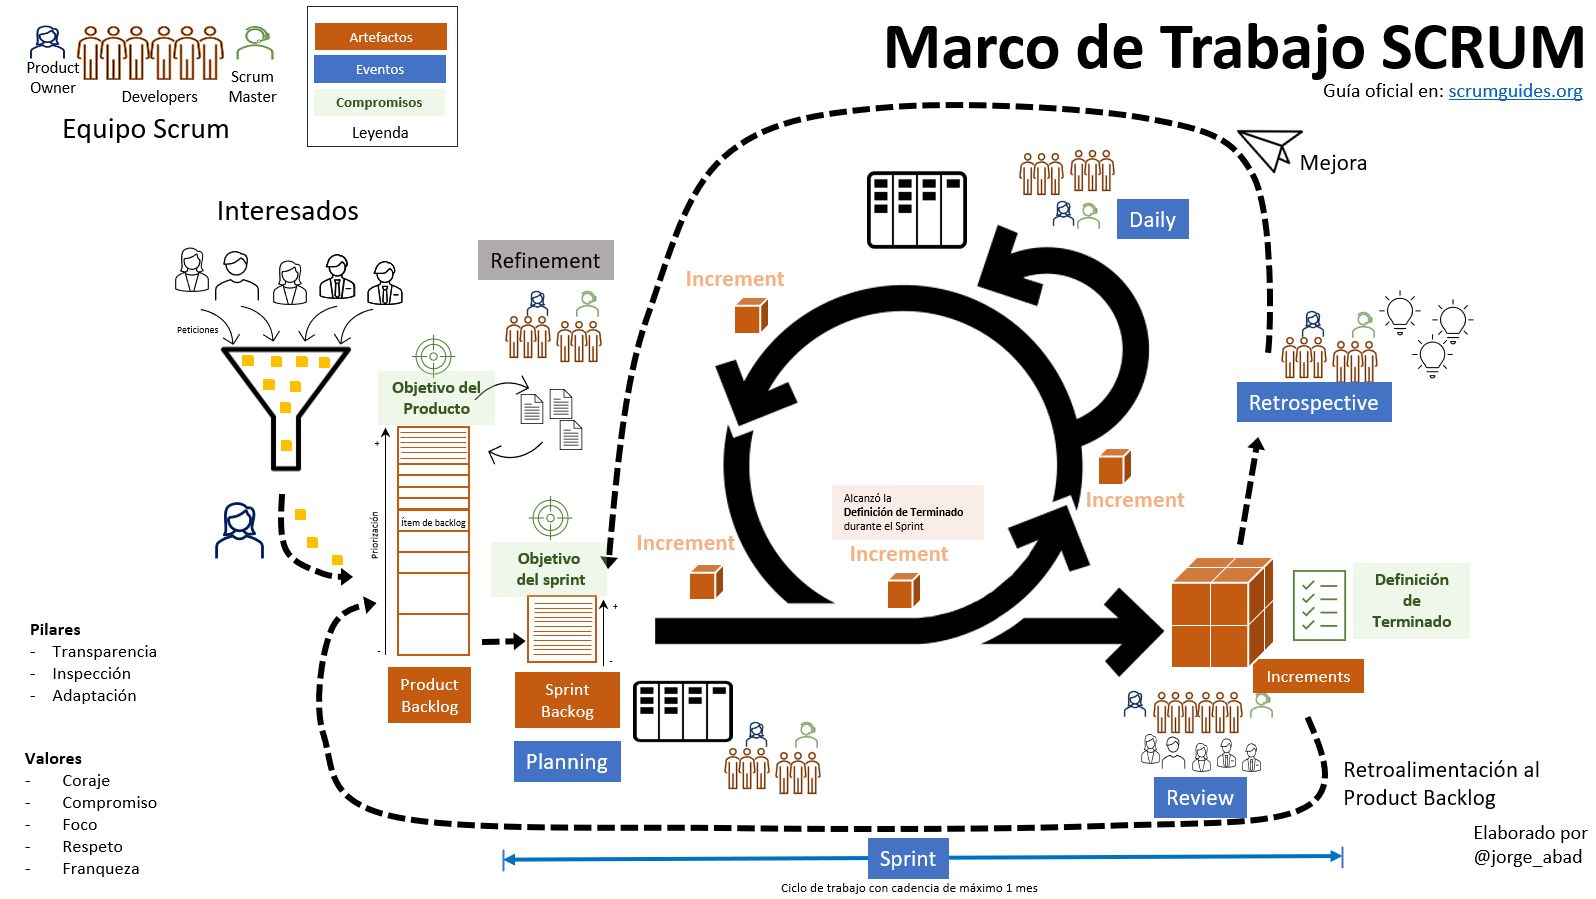
\includegraphics[width=0.8\textwidth]{assets/scrum-diagram.png}
  \caption{Diagrama del proceso completo de Scrum (\href{https://www.lecciones-aprendidas.info/2023/09/diagrama-explicativo-scrum-guia-2020.html}{Fuente})}
  \label{fig:scrum-diagram}
\end{figure}

En esta imagen podemos ver definido todo el proceso que se sigue con una metodología Scrum, desde la planificación del producto hasta la entrega del mismo.

Tal y como se comenta en la guía de Scrum y podemos ver en la imagen, durante el desarrollo del proyecto se van a generar varios artefactos:
\begin{itemize}
    \item \textbf{Product Backlog}: es una lista priorizada de requisitos o tareas pendientes en un proyecto ágil. En este caso, el product backlog se va a utilizar para organizar todas las historias de usuario e historias técnicas que se van a implementar en el proyecto.
    \item \textbf{Sprint Backlog}: es una lista de tareas (las cuales salen de las historias de usuario y técnicas) seleccionadas del product backlog que se van a realizar durante un sprint.
    \item \textbf{Incremento}: es la suma de todos los elementos del product backlog completados durante un sprint y los incrementos de todos los sprints anteriores. En este caso, el incremento se va a utilizar para organizar todas las tareas que se han realizado durante cada sprint.
\end{itemize}
De esta manera buscamos al tener un objetivo de producto claro y definido en los sprints. Aunque el producto sufra cambios después, queremos intentar estimar lo mejor posible y, sobre todo, terminar los sprints con un producto con \textbf{valor}, tal y como se dice en la guía `\textit{A product is a vehicle to deliver value. It has a clear boundary, known stakeholders, well-defined users or customers. A product could be a service, a physical product, or something more abstract.}'

Separaremos el desarrollo en distintos sprints, cada uno de ellos con una duración de dos semanas.

Durante cada sprint se seleccionarán las historias de usuario\footnote{Las historias de usuario son descripciones concisas y sencillas de una funcionalidad, escritas desde la perspectiva del usuario} al principio del sprint y se desarrollarán (posible desglose en distintas historias de usuario, definición de tareas relacionadas con la HU junto con estimación de las mismas y definición de pruebas de aceptación) generando así el Sprint Backlog correspondiente a ese sprint, se completarán las tareas necesarias para completarlas.

Al final del sprint se realizará una revisión en la que se analizará lo que se ha conseguido hacer y si hemos cumplido con lo que habíamos definido antes del sprint para adaptar el product backlog si fuera necesario y tenerlo en cuenta para el siguiente sprint. En la revisión participarán Product Owner, equipo de desarrollo, Scrum Master y los interesados en el proyecto (Stakeholders). Aquí es donde se presenta el incremento del producto a los interesados y se recibe retroalimentación sobre el trabajo realizado.

Y por último se lleva a cabo una retrospectiva en el equipo, donde se reflexiona principalmente sobre el cómo se ha trabajado, qué se ha hecho bien, qué se ha hecho mal y qué se puede mejorar para el siguiente sprint. Esto es una parte fundamental de Scrum, ya que permite al equipo aprender de su experiencia y mejorar continuamente.

Gracias a esta metodología conseguimos tener una organización muy clara de lo que se va a hacer, cómo se va a hacer y cuándo se va a hacer.

\subsection{Tecnologías}
% TODO: Relacionar con los requisitos/objetivos.
Para el desarrollo de este proyecto se ha buscado utilizar tecnologías que sean lo más eficientes y rápidas posibles, pero a la vez que sean seguras y escalables. Se ha buscado un equilibrio entre rendimiento y facilidad de uso, ya que el objetivo principal es conseguir un producto funcional y eficiente.

\subsubsection{Servidor}
Para la parte de servidor se va a hacer uso de uno de los lenguajes más venerados en la actualidad en el mundo de la programación: \textbf{Rust}.

Rust es un lenguaje de programación de sistemas que se centra en la seguridad, el rendimiento y la concurrencia. Se ha convertido en una opción popular para el desarrollo de aplicaciones de alto rendimiento y sistemas críticos.
Aunque Rust es un lenguaje de bajo nivel, su sintaxis es muy similar a la de otros lenguajes de programación como C++ o Java, lo que facilita su aprendizaje para los programadores que ya tienen experiencia en estos lenguajes, permitiendo un desarrollo más seguro, rápido y eficiente. 

¿Por qué la elección de este lenguaje para el desarrollo del servidor de sincronización? \parencite{rust-for-safety-and-performance}
\begin{itemize}
    \item \textbf{Rendimiento}: es conocido por su alto rendimiento, lo que lo convierte en una excelente opción para aplicaciones que requieren un procesamiento intensivo de datos. Aunque es un lenguaje enfocado a sistemas, el rendimiento de sus librerías para desarrollo web es muy bueno, como se puede ver en distintos benchmark \parencite{rust-benchmark}.
    \item \textbf{Seguridad}: tiene un sistema de tipos y un modelo de propiedad que ayudan a prevenir errores comunes de programación, como desbordamientos de búfer y condiciones de carrera.
    \item \textbf{Concurrencia}: soporta de manera nativa y sencilla la escritura de código concurrente y paralelo, lo que es esencial para aplicaciones que manejan múltiples tareas al mismo tiempo.
        Gracias a su implementación de \gls{fearless-concurrency}, Rust permite a los desarrolladores escribir código concurrente sin preocuparse por errores comunes como condiciones de carrera o deadlocks, lo que facilita la creación de aplicaciones altamente eficientes y escalables.
    \item \textbf{Manejo de errores}: tiene un enfoque único para el manejo de errores, utilizando tipos de datos como \texttt{Result} y \texttt{Option} para representar resultados exitosos y fallidos, lo que ayuda a evitar errores en tiempo de ejecución, consiguiendo de esta manera no encontrarnos con errores inesperados a la hora de ejecutar la aplicación.
    \item \textbf{Ecosistema}: cuenta con un ecosistema en crecimiento, con una amplia variedad de bibliotecas y herramientas que facilitan el desarrollo de aplicaciones.
\end{itemize}


\begin{figure}[H]
  \centering
  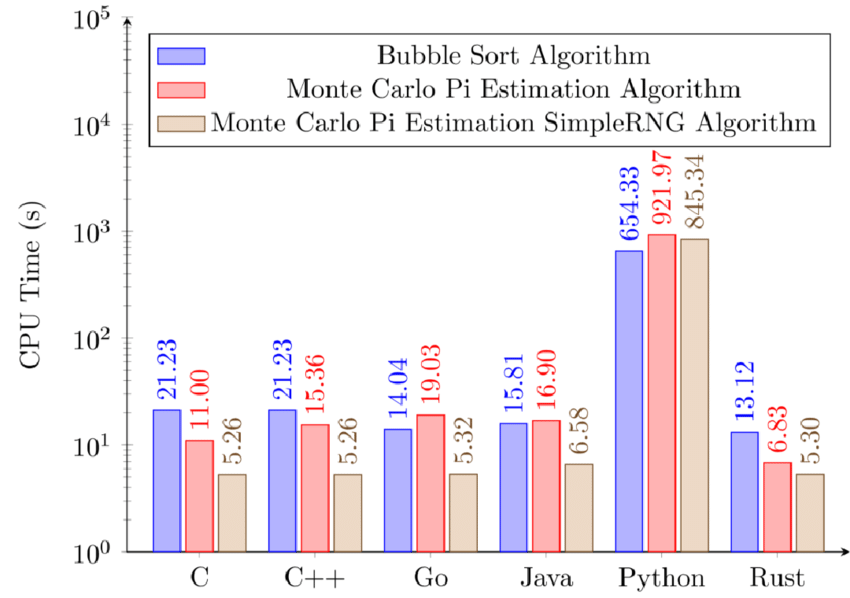
\includegraphics[width=0.8\textwidth]{assets/rust-cpu-comparison.png}
  \caption{Comparativa de uso de CPU entre Rust y otros lenguajes de programación (menos es mejor) \parencite{rust-for-safety-and-performance}}
  \label{fig:rust-cpu-comparison}
\end{figure}


\begin{figure}[H]
  \centering
  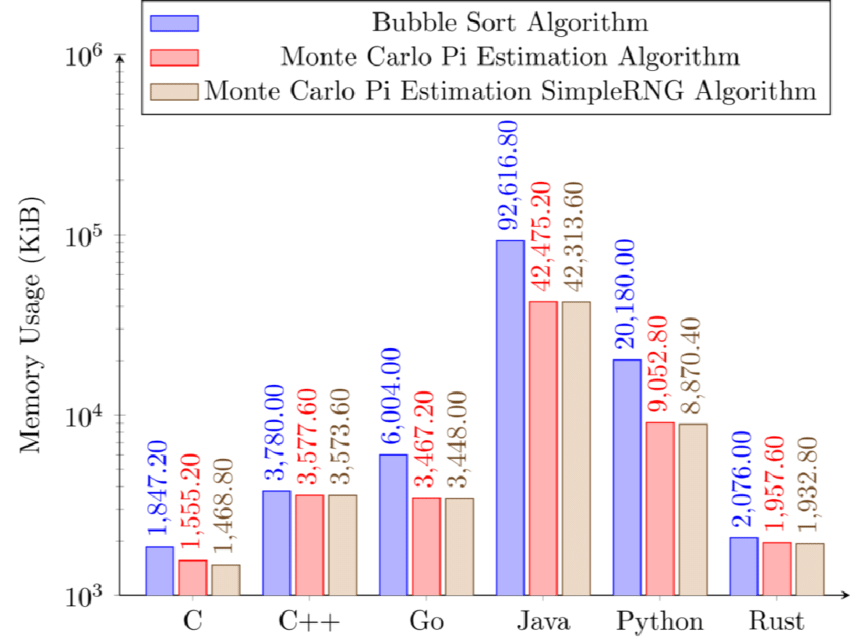
\includegraphics[width=0.8\textwidth]{assets/rust-memory-comparison.png}
  \caption{Comparativa de uso de memoria entre Rust y otros lenguajes de programación (menos es mejor) \parencite{rust-for-safety-and-performance}}
  \label{fig:rust-memory-comparison}
\end{figure}

Como se puede ver en las figuras \ref{fig:rust-cpu-comparison} y \ref{fig:rust-memory-comparison}, Rust tiene un rendimiento muy bueno en comparación con otros lenguajes de programación, tanto en uso de CPU como en uso de memoria.

A partir de las figuras, podemos definir dos fórmulas para calcular el porcentaje de mejora con respecto a los otros lenguajes de programación:
\begin{equation}
    \text{Mejora}_{\text{CPU}} (\%) = \left( \frac{T_{\text{\textit{lenguaje}}} - T_{\text{Rust}}}{T_{\text{\textit{lenguaje}}}} \right) \times 100
\end{equation}

\begin{equation}
    \text{Mejora}_{\text{Memoria}} (\%) = \left( \frac{M_{\text{\textit{lenguaje}}} - M_{\text{Rust}}}{M_{\text{\textit{lenguaje}}}} \right) \times 100
\end{equation}


Obteniendo las siguientes tablas de comparación:

\begin{table}[H]
\centering
\begin{tabular}{|c|c|c|c|}
\hline
\textbf{Lenguaje} & \textbf{Bubble Sort} & \textbf{Monte Carlo Pi} & \textbf{Monte Carlo Pi (SimpleRNG)} \\
\hline
C      & 38.2\%  & 37.9\%  & -0.8\% \\
C++    & 38.2\%  & 55.5\%  & -0.8\% \\
Go     & 6.5\%   & 64.1\%  & 0.4\%           \\
Java   & 17.0\%  & 59.6\%  & 19.4\%          \\
Python & 98.0\%  & 99.3\%  & 99.4\%          \\
\hline
\end{tabular}
\caption{Porcentaje de mejora de Rust con respecto a otros lenguajes de programación en términos de tiempo de CPU. (Mayor es mejor)}
\end{table}

\begin{table}[H]
\centering
\begin{tabular}{|c|c|c|c|}
\hline
\textbf{Lenguaje} & \textbf{Bubble Sort} & \textbf{Monte Carlo Pi} & \textbf{Monte Carlo Pi (SimpleRNG)} \\
\hline
C      & 89.8\%  & 20.4\%  & 25.6\%  \\
C++    & 45.1\%  & 45.3\%  & 45.9\%  \\
Go     & 65.4\%  & 43.5\%  & 44.0\%  \\
Java   & 97.8\%  & 95.4\%  & 95.4\%  \\
Python & 89.7\%  & 78.4\%  & 78.2\%  \\
\hline
\end{tabular}
\caption{Porcentaje de mejora de Rust con respecto a otros lenguajes de programación en términos de uso de memoria. (Mayor es mejor)}
\end{table}

Haremos uso del framework de aplicaciones web \href{https://github.com/tokio-rs/axum?tab=readme-ov-file}{\textbf{Axum}}.

Axum es un framework de aplicaciones web construido sobre Tokio, una biblioteca de programación asíncrona para Rust. Axum se centra en la simplicidad y la facilidad de uso, lo que lo convierte en una excelente opción para desarrollar aplicaciones web rápidas y eficientes.
Aunque hay varios frameworks más eficientes en términos de velocidad a la hora de realizar benchmarks\footnote{\href{https://web-frameworks-benchmark.netlify.app/result?l=rust}{Comparativa frameworks de Rust}} \footnote{\href{https://www.techempower.com/benchmarks/\#section=data-r21&test=composite&hw=ph}{Comparativa con frameworks de otros lenguajes}}, algunos de ellos tienen un tiempo de compilación demasiado alto, por lo que puede llegar a hacer más lento el desarrollo.
Además, ninguno de los demás frameworks de Rust tiene una comunidad tan activa como la de Axum ni una documentación tan completa.

Axum al estar desarrollado sobre la librería de Tokio\footnote{Librería de Rust más usada para la programación asíncrona}, garantiza un soporte a largo plazo que otros frameworks no garantizan. Además, es \href{https://lib.rs/crates/axum}{la librería más descargada }mensualmente para aplicaciones web en Rust.  

Como se puede ver en los benchmark hay frameworks de otros lenguajes que pueden parecer más sencillos que Rust que nos dan el mismo o mejor rendimiento, pero tal y como se ha comentado anteriormente, el punto principal de Rust no es únicamente su rendimiento, sino la seguridad que da el propio lenguaje y lo poco propenso que es a errores en tiempo de compilación, lo que hace de la aplicación mucho más robusta, segura y sostenible a largo plazo.


\subsubsection{Móvil}
Para el desarrollo de la aplicación móvil se ha optado por un nuevo framework de desarrollo multiplataforma, \textbf{Lynx.js}.

Lynx.js es un framework inspirado en React Native. El desarrollo de la aplicación se hace con React el cual se compila a código nativo de la plataforma. El framework soporta componentes de cualquier framework de desarrollo web, aunque está pensado para usar React y es lo que usaremos nosotros.

Aunque pueda parecer igual que React Native, Lynx añade algunas cosas que le faltan a React Native. Uno de los mayores problemas de React Native es su rendimiento en algunas situaciones, ya que este solamente hace uso de un solo thread, lo cual no permite una buena gestión de las tareas. Por ejemplo, no puede obtener datos de una API mientras que se actualiza lo que se muestra al usuario.

Sin embargo, Lynx tiene dos threads, un main thread y un background thread.
Gracias a esto, es posible especificar en qué thread se va a ejecutar cada función, consiguiendo de esta manera que tareas como mostrar rápidamente la interfaz se hagan lo más rápido posible mientras que en el background thread se obtienen los datos de la API.
Esto da una experiencia al usuario mucho más fluida y rápida, principalmente gracias a el \gls{ifr} (\acrshort{ifracr}).

Para conseguir esto, Lynx altera el ciclo de vida de los componentes de React (figura \ref{fig:lynx-component-lifecycle}), consiguiendo deshacerse de cuellos de botella típicos que aparecen en los frameworks de desarrollo móvil asegurando un rendimiento óptimo y una experiencia de usuario fluida.

\begin{figure}[h]
    \begin{center}
        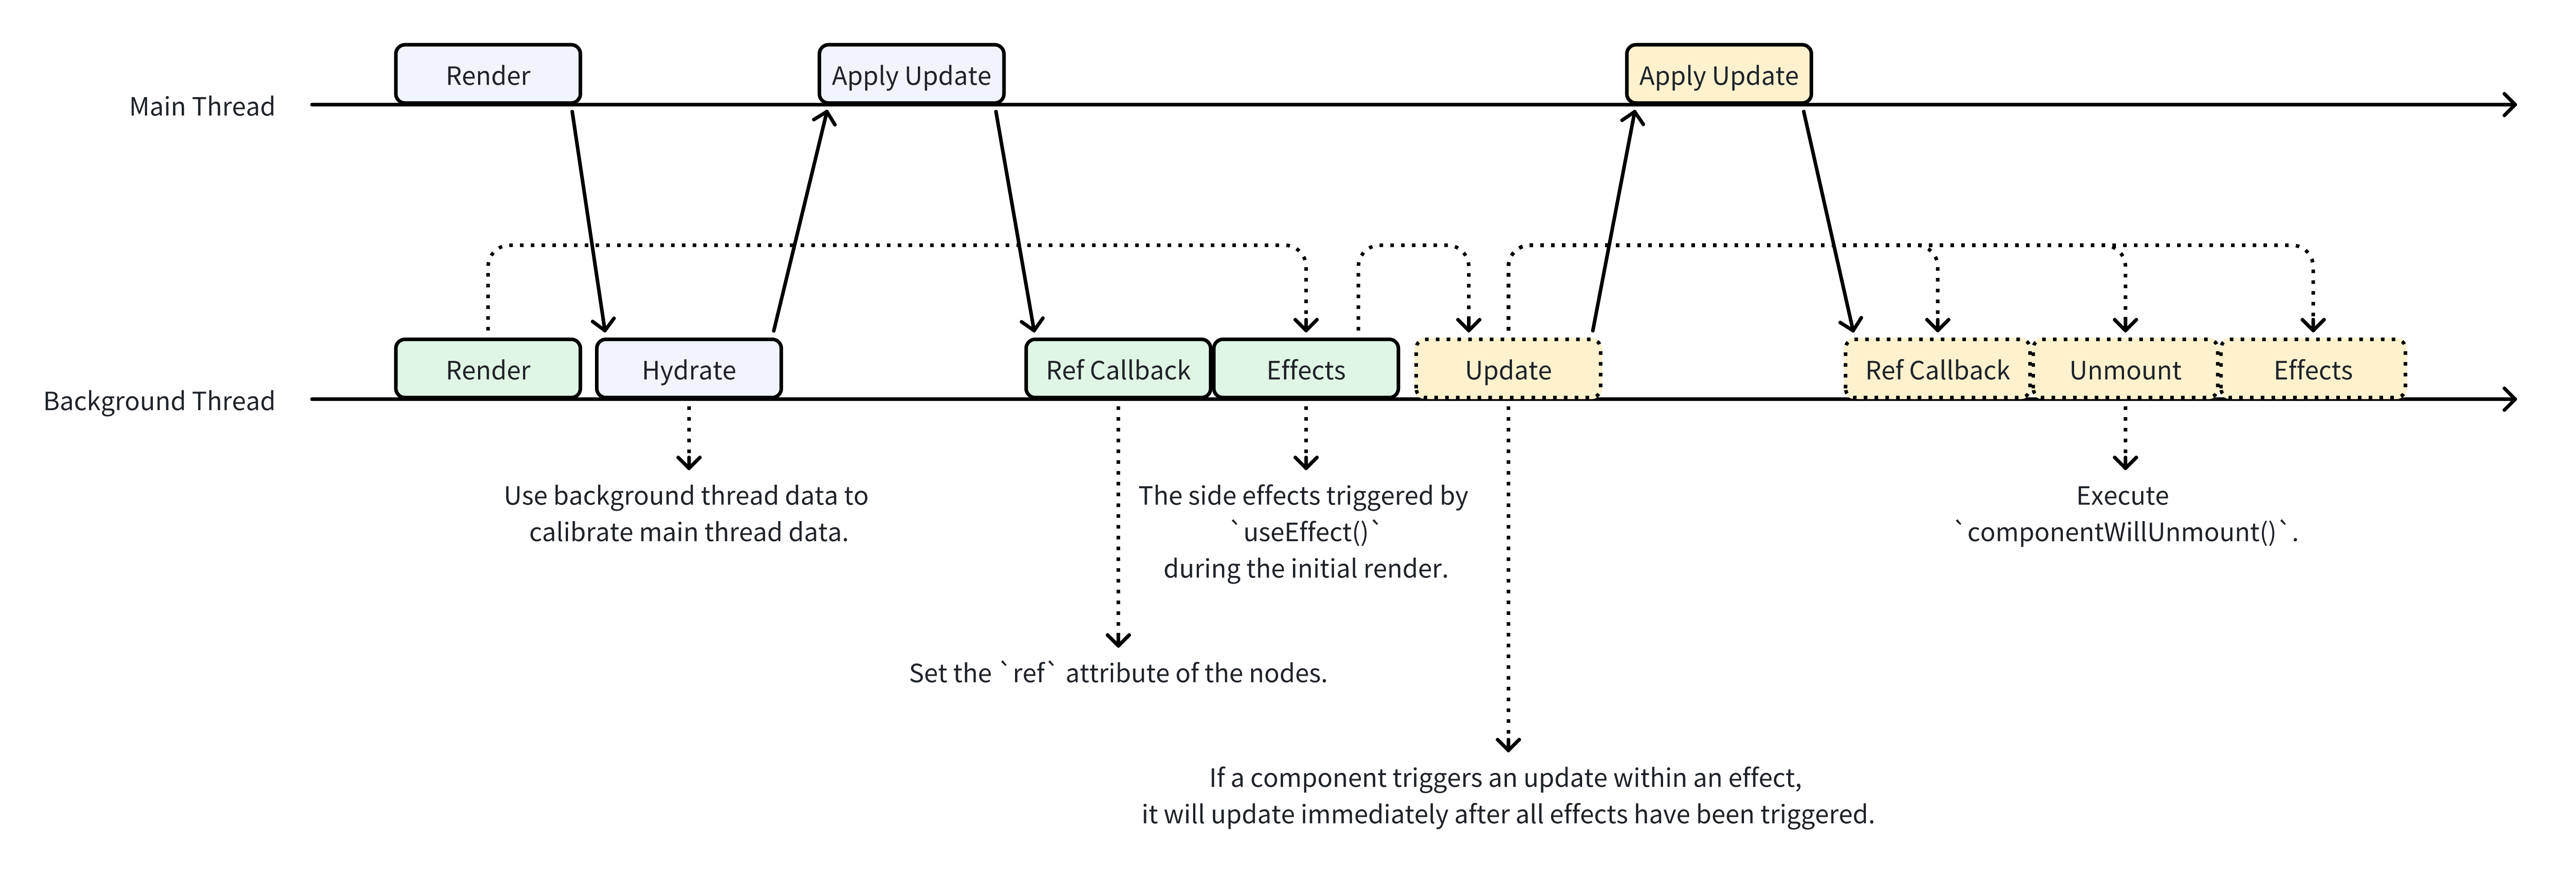
\includegraphics[width=\textwidth]{lynx-lifecycle.png}
    \end{center}
    \caption{Ciclo de vida de los componentes en Lynx.js (\href{https://lynxjs.org/react/lifecycle.html}{Documentación})}
    \label{fig:lynx-component-lifecycle}
\end{figure}


Dado que la aplicación necesitará hacer uso de módulos nativos de los teléfonos, necesitaremos implementarlos para cada plataforma.
Esto se puede hacer de manera sencilla, ya que el framework permite la creación de módulos nativos los cuales se pueden llamar desde nuestro código escrito en React.

Este es uno de los puntos fuertes de la aplicación, ya que nos va a permitir programar haciendo uso de React, el cual es un framework muy conocido y utilizado, pero a la vez nos va a permitir hacer uso de módulos nativos de cada plataforma, lo que nos da una gran flexibilidad a la hora de desarrollar la aplicación de forma nativa en todas las plataformas.

Lynx usa una aplicación nativa \textit{Lynx Explorer}, con la cual podemos ver cómo se va a ver la aplicación en el dispositivo móvil. Esta aplicación es la que se encarga de compilar el código de Lynx a código nativo y de ejecutar la aplicación en el dispositivo móvil.
Para poder hacer uso de los módulos nativos, tendremos que implementarlos en el Explorer, un proyecto que implementa el runtime que utiliza Lynxjs por debajo tanto en Android como iOS, compilar el código del mismo y una vez tenemos la aplicación con nuestro módulo nativo, podemos ejecutar nuestra aplicación sobre nuestro Explorer y hacer uso de nuestro módulo nativo.

A la hora de compilar nuestra aplicación para ser usada en producción, Lynx se incorpora sobre un SDK de Android o iOS. Gracias a esto podemos incorporar nuestra aplicación en cualquier otra aplicación existente con tan solo compilar nuestro código y añadirlo con el SDK de Lynx en la plataforma que gustemos.
En nuestro caso nos limitamos a usar una estructura de aplicación que proporcionan en \href{https://github.com/lynx-family/integrating-lynx-demo-projects}{su repositorio oficial de proyectos de ejemplo}, los cuales contienen proyectos vacíos que hacen uso de el SDK correspondiente en cada plataforma, por lo que tan solo tendremos que incorporar nuestra aplicación hecha con Lynx.js compilada y compilar el proyecto para cada plataforma.

El proceso de compilación de una aplicación para producción sigue siendo complejo aún, ya que tal y como he comentado, Lynx.js no tiene aún una manera definitiva de compilar un proyecto sin tener que integrarlo mediante el SDK de Lynx en un proyecto nativo de Android o iOS. Aún así, el repositorio con los proyectos de ejemplo proporciona una buena base para empezar a trabajar con Lynx.js y nos permite centrarnos en el desarrollo de la aplicación sin tener que preocuparnos por la configuración del proyecto.

Todo esto, junto con los comandos y repositorios necesarios viene detallado en el artículo hecho por el equipo de Lynx \parencite{lynx-native-modules}.

Dado que para el desarrollo de aplicaciones en iOS es necesario tener un sistema de Apple, en la implementación de esta aplicación nos centraremos en la parte de Android, aunque el código de la aplicación será el mismo para ambas plataformas.
La única diferencia será la implementación de los módulos nativos, que serán diferentes para cada plataforma.

En resumen, las ventajas de usar este framework con respecto a otros son:
\begin{itemize}
    \item \textbf{Rendimiento}: al compilar a código nativo, el rendimiento es mucho mejor que el de otros frameworks como Flutter. Además, Lynx nos permite hacer uso de su tecnología de doble thread, haciendo que nuestra aplicación sea mucho más fluida y rápida en comparación con otras tecnologías.
    \item \textbf{Flexibilidad}: permite la creación de módulos nativos para cada plataforma, lo que da una gran flexibilidad a la hora de desarrollar la aplicación.
    \item \textbf{Simplicidad}: la sintaxis es muy similar a la de React, lo que facilita su aprendizaje para los programadores que ya tienen experiencia en este framework.
    \item \textbf{Documentación}: la documentación es muy completa y está en constante actualización.
\end{itemize}

¿Por qué no se ha optado por otras opciones como Flutter o Kotlin Multiplatform?
\begin{itemize}
    \item \textbf{Flutter}: aunque es un framework muy potente y con una comunidad muy activa, su rendimiento no es tan bueno como el de Lynx.js. 
        Flutter lo que hace es renderizar lo que sería como un ``canvas'' que utiliza un motor gráfico parecido al de los juegos para renderizar la interfaz de usuario, haciendo que la experiencia de usuario no sea tan fluida como podría ser la de otro framework. 
    \item \textbf{Kotlin Multiplatform}: aunque es una opción interesante, la comunidad y la documentación son mucho más limitadas que las de Lynx.js. La curva de aprendizaje es mucho más pronunciada, ya que se utiliza Kotlin junto con una gran cantidad de librerías las cuales necesitan de un estudio profundo para su uso.

        Nos daría el mejor rendimiento sin tener que programar la aplicación de forma nativa para todos los dispositivos (los dispositivos comparten código pero hay que implementar la mayoría de forma nativa para las distintas plataformas), pero el desarrollo sería mucho más lento y tedioso, lo cual además complicaría la aportación al proyecto Open Source.
    \item \textbf{React Native}: aunque es un framework muy conocido y utilizado, su rendimiento no es tan bueno como el de Lynx.js.
        Es una opción muy parecida a Lynx.js, pero a largo plazo la aplicación podría verse afectada por el rendimiento.
        Dada la similitud con Lynx.js y las ventajas que ofrece, se ha optado por este último.
\end{itemize}

Este framework ha sido desarrollado de cero por el equipo de TikTok. Es utilizado por ellos para el desarrollo de varias de sus aplicaciones, por lo que aunque ha cambiado a ser Open-Source hace poco con su versión 3.2.0, es un framework que ya ha sido probado en producción en aplicaciones como \textbf{TikTok Studio}, \textbf{Disney100 en TikTok}, \textbf{The Met Gala en TikTok} tal y como comentan en el artículo en el que anunciaron que Lynx.js pasaba a ser Open-Source \parencite{lynx-article}.

\subsection{Historias de usuario / Historias técnicas}
\label{sec:historias-de-usuario}
En esta sección se detallan las historias de usuario e historias técnicas de la aplicación, separadas en dos grupos: las de la aplicación de servidor y las de móvil.

Se ha considerado esta separación ya que la aplicación de servidor tiene un objetivo diferente al de la aplicación móvil, de esta manera conseguimos una mejor organización de las historias de usuario.

Durante los primeros sprints se trabajará de manera principalmente separada, enfocándose en la parte correspondiente que se defina de la aplicación y en una fase más avanzada se trabajará de manera conjunta, integrando ambas aplicaciones. Esto lo hacemos para para poder enfocarnos mejor en una sola parte del proyecto, de esta manera no tenemos que estar cambiando de contexto constantemente entre las dos aplicaciones, lo que podría hacer que el desarrollo fuera más lento y tedioso.

Para la planificación del desarrollo se han utilizado puntos de historia (PH), los cuales representan una estimación de lo que se considera que se tardará en implementar las historias de usuario. Esta estimación es relativa, es decir, no representa un tiempo real sino una estimación con respecto a todas las demás historias de usuario, siendo 1 punto de historia la historia de usuario más sencilla de implementar o que menos tiempo requiere.

Este es un listado inicial de historias de usuario, durante los sprints se irá especificando si alguna historia de usuario ha cambiado, añadido o eliminado del product backlog\footnote{El product backlog es una lista priorizada de requisitos o tareas pendientes en un proyecto ágil.}.

Cada historia de usuario tiene un identificador único, una descripción de la historia de usuario y una estimación en puntos de historia. Ésta es después desglosada en historias de usuario más pequeñas de las cuales se definen tareas que tienen que ser realizadas para completar la historia de usuario con su estimación en horas.
Además de las historias de usuario, contamos con historias técnicas, que son historias de usuario que no están relacionadas directamente con el usuario final, sino que son necesarias para el correcto funcionamiento del sistema. Estas historias técnicas se consideran como historias de usuario y se les asigna una estimación en puntos de historia.

A lo largo del product backlog  se hará referencia a HU\{identificador\} para las historias de usuario y HT\{identificador\} para las historias técnicas. El identificador será un número entero que se asignará de manera consecutiva a cada historia de usuario o historia técnica. Para la sub-historias de usuario se asignará un número entero que será el mismo que la historia de usuario a la que pertenece, seguido de un punto y otro número entero que será el identificador de la sub-historia de usuario, por ejemplo: HU1, HU1.1, HU1.2, etc.

\subsubsection{Servidor}
\renewcommand{\arraystretch}{1.3} % Increases row height for readability
\rowcolors{2}{gray!15}{white} % Alternate row colors

\begin{tabularx}{\textwidth}{|l|l|>{\raggedright\arraybackslash}X|l|}
    \hline
\textbf{ID} & \textbf{Título} & \textbf{Descripción} & \makecell{\textbf{Estimación}\\\textbf{(PH)}} \\
    \hline
    HU01 & Subida de fotos & Como usuario, quiero subir varias fotos desde mi móvil para tener una copia de seguridad en mi servidor. & 5 \\
    \hline
    HU02 & Estado de sincronización & Como usuario, quiero ver qué fotos están subidas y cuáles no, para saber el estado de sincronización. & 3 \\
    \hline
    HU03 & Eliminar fotos & Como usuario, quiero eliminar fotos subidas desde la app, para liberar espacio en mi servidor. & 3 \\
    \hline
    HU04 & Subida de vídeos & Como usuario, quiero subir vídeos además de fotos, para guardar también mis recuerdos en vídeo. & 5 \\
    \hline
    HU05 & Inicio de sesión & Como usuario, quiero iniciar sesión con contraseña o clave, para evitar que otros accedan a mis archivos. & 5 \\
    \hline
    HU06 & Cerrar sesión & Como usuario, quiero poder cerrar sesión en un dispositivo, para proteger mis datos si pierdo el móvil. & 2 \\
    \hline
    HU07 & Descubrimiento automático & Como usuario, quiero que la app detecte automáticamente mi servidor en la red local, para no tener que configurarlo manualmente. & 8 \\
    \hline
    HU08 & Conexión remota & Como usuario, quiero poder conectarme remotamente si expongo mi servidor, para acceder a mis fotos desde fuera de casa. & 13 \\
    \hline
    HU09 & Galería visual & Como usuario, quiero ver una galería de las fotos y videos subidos, para revisar mi contenido fácilmente. & 5 \\
    \hline
    HU10 & Espacio ocupado & Como usuario, quiero ver el espacio ocupado por mis archivos, para controlar el almacenamiento del servidor. & 3 \\
    \hline
    HU11 & Estadísticas de copia & Como usuario, quiero ver estadísticas de sincronización, para saber cuándo fue la última copia y cuántos archivos se han guardado. & 3 \\
    \hline
    HU12 & Cancelar sincronización & Como usuario, quiero cancelar una sincronización en curso. & 5 \\
    \hline
    HU13 & Crear cuentas & Como administrador, quiero crear cuentas de usuario con permisos, para que varias personas puedan usar el servidor. & 8 \\
    \hline
    HU14 & Galería privada & Como usuario, quiero tener mi propia galería separada de otros usuarios. & 5 \\
    \hline
    HU15 & Galería online & Como usuario, quiero poder ver todas las fotos que tengo en el servidor sin necesidad de tener que descargarlas en mi móvil, tanto las que he subido yo como las que han compartido conmigo. & 8 \\
    \hline
    HT01 & Hash de archivos & Implementar sistema de cálculo de hash para detectar duplicados. & 3 \\
    \hline
    HT02 & Sincronización incremental & Implementar sincronización basada en metadatos (fecha, tamaño, hash). & 5 \\
    \hline
    HT03 & API REST en Rust & Desarrollar API RESTful usando Rust y Axum & 13 \\
    \hline
    HT04 & Descubrimiento mDNS & Crear sistema de descubrimiento automático usando mDNS. & 8 \\
    \hline
    HT05 & Autenticación JWT & Implementar autenticación con JSON Web Tokens. & 5 \\
    \hline
    HT06 & HTTPS en servidor & Configurar comunicación segura con HTTPS. & 5 \\
    \hline
    HT07 & Estructura de almacenamiento & Definir carpetas y metadatos para organizar los archivos. & 5 \\
    \hline
    HT08 & Base de datos & Implementar SQLite o PostgreSQL para usuarios y archivos. & 8 \\
    \hline
    HT09 & Compresión de imágenes & Implementar compresión para optimizar el almacenamiento. & 5 \\
    \hline
    HT10 & Subida concurrente & Soporte para subida simultánea y manejo de errores. & 8 \\
    \hline
    HT11 & Tests en Rust & Añadir pruebas unitarias e integración en backend. & 5 \\
    \hline
    HT12 & CI/CD & Configurar pipelines de integración y despliegue. & 5 \\
    \hline
    HT13 & Logging & Implementar logs detallados para depuración. & 3 \\
    \hline
    HT14 & Cobertura de tests & Medir y asegurar la cobertura de pruebas. & 3 \\
    \hline
    HT15 & Interfaz Tauri & Crear interfaz gráfica del servidor con Tauri. & 8 \\
    \hline
    HT16 & Panel de control & Implementar visualización de archivos y uso del sistema. & 5 \\
    \hline
    HT17 & Notificaciones de progreso & Integrar notificaciones del sistema con progreso de subida. & 3 \\
    \hline
    HT18 & Binario y Tauri & Empaquetar servidor como CLI y app Tauri. & 5 \\
    \hline
    HT19 & Dockerización & Crear imagen Docker del servidor. & 3 \\
    \hline
    HT20 & Documentación & Documentar instalación y uso del sistema. & 13 \\
    \hline
    HT21 & Backups externos & Soporte para backups automáticos externos. & 8 \\
    \hline
    HT22 & Logs persistentes & Configurar sistema de logs persistentes y rotación. & 3 \\
    \hline
\end{tabularx}

\paragraph{Historias que se han dividido}

\begin{table}[H]
    \begin{center}
        \begin{tabularx}{\textwidth}{|l|l|>{\raggedright}X|l|}
            \hline
            ID & Título & Descripción & Estimación \\
            \hline
            HT18 & Binario y Tauri & Empaquetar servidor como CLI y app Tauri. & 5 \\
            \hline
            HT18.1 & Binario & Empaquetar la aplicación como un solo binario & 2 \\
            \hline
            HT18.2 & Tauri & Empaquetar aplicación de escritorio con Tauri & 3 \\
            \hline
        \end{tabularx}
    \end{center}
\end{table}

\begin{table}[H]
    \begin{center}
        \begin{tabularx}{\textwidth}{|l|X|>{\raggedright\arraybackslash}X|l|}
            \hline
            ID & Título & Descripción & Estimación \\
            \hline
            HT20 & Documentación & Documentar instalación y uso del sistema. & 13 \\
            \hline
            HT20.1 & Documentación del proyecto en Github & Documentar la instalación y uso del proyecto en el repositorio de Github & 5 \\
            \hline
            HT20.2 &  Documentación de la API REST con OpenAPI & Documentar mediante la generación de una página web todos los endpoints de la API REST & 5 \\
            \hline
            HT20.3 & Documentación de la aplicación Tauri & Manual de usuario de la aplicación de escritorio desarrollada con Tauri & 3 \\
            \hline
        \end{tabularx}
    \end{center}
\end{table}

\newpage
\subsubsection{Móvil} 
\begin{tabularx}{\textwidth}{|l|l|>{\raggedright\arraybackslash}X|l|}
    \hline
    ID & Título & Descripción & Estimación \\
    \hline
    HU16 & Seleccionar fotos & Como usuario, quiero seleccionar varias fotos desde mi galería para subirlas al servidor. & 3 \\
    \hline
    HU17 & Subir fotos automáticamente & Como usuario, quiero que se suban automáticamente las nuevas fotos que hago, sin tener que hacerlo manualmente. & 8 \\
    \hline
    HU18 & Ver progreso de subida & Como usuario, quiero ver el progreso de cada archivo que se está subiendo. & 8 \\
    \hline
    HU19 & Cancelar subida & Como usuario, quiero cancelar una subida en curso desde la interfaz. & 3 \\
    \hline
    HU20 & Ver archivos subidos & Como usuario, quiero ver una lista o galería de los archivos que ya están subidos. & 5 \\
    \hline
    HU21 & Conexión automática al servidor & Como usuario, quiero que la app detecte y se conecte automáticamente al servidor en mi red. & 5 \\
    \hline
    HU22 & Cambiar de servidor & Como usuario, quiero poder cambiar manualmente la dirección del servidor si quiero usar otro. & 3 \\
    \hline
    HU23 & Ver uso de almacenamiento & Como usuario, quiero ver cuánto espacio he usado en el servidor. & 3 \\
    \hline
    HU24 & Inicio y cierre de sesión & Como usuario, quiero iniciar y cerrar sesión para proteger mis datos. & 5 \\
    \hline
    HU25 & Gestión de permisos & Como usuario, quiero que la app me pida permisos de acceso solo cuando sea necesario. & 3 \\
    \hline
    HU26 & Notificaciones de subida & Como usuario, quiero recibir notificaciones cuando se complete la sincronización. & 5 \\
    \hline
    HU27 & Subir vídeos & Como usuario, quiero subir también vídeos de mi galería al servidor. & 5 \\
    \hline
    HU28 & Subida en segundo plano & Como usuario, quiero que las subidas continúen aunque cierre la app. & 8 \\
    \hline
    HU29 & Sincronización manual & Como usuario, quiero poder iniciar la sincronización manualmente. & 3 \\
    \hline
    HU30 & Galería online & Como usuario, quiero ver mis fotos en la app sin tener que descargarlas. & 5 \\
    \hline
    HT23 & Acceso a la galería & Implementar acceso seguro a la galería de fotos y vídeos. & 5 \\
    \hline
    HT24 & Comunicación con API & Integrar cliente HTTP que se comunique con el servidor. & 5 \\
    \hline
    HT25 & Almacenamiento local & Guardar estado de archivos subidos/no subidos de forma local. & 3 \\
    \hline
    HT26 & Manejo de errores de red & Implementar gestión de errores de red y reintentos automáticos. & 5 \\
    \hline
    HT27 & Subida concurrente & Soportar subida de varios archivos en paralelo con control de errores. & 5 \\
    \hline
    HT28 & Sincronización de fondo & Implementar sincronización en segundo plano. & 8 \\
    \hline
    HT29 & Pruebas unitarias & Añadir pruebas unitarias y de integración a la lógica común en React Native / Lynx.js & 13 \\
    \hline
    HT30 & CI/CD móvil & Pipeline de construcción y publicación para Android e iOS. & 5 \\
    \hline
    HT31 & Gestión de tokens & Almacenar y renovar tokens de autenticación de forma segura. & 3 \\
    \hline
    HT32 & Notificaciones locales & Integrar sistema de notificaciones locales en Android/iOS. & 3 \\
    \hline
    HT33 & Optimización de red & Reducir uso de red usando compresión. & 5 \\
    \hline
    HT34 & Localización & Soporte multilenguaje para la aplicación. & 8 \\
    \hline
    HT35 & Permisos condicionales & Solicitar permisos en tiempo de ejecución de forma contextual. & 3 \\
    \hline
    HT36 & UI responsive & Adaptar UI para distintos tamaños de pantalla (tablet, móvil). & 3 \\
    \hline
\end{tabularx}

\subsection{Planificación inicial}
\label{sec:planificacion-inicial}
Durante un desarrollo con Scrum, tal como se ha comentado anteriormente en la \hyperref[sec:metodologia]{sección de metodología}, se usan \textbf{sprints} para dividir el desarrollo en partes organizadas y planificadas con anterioridad, las cuales tienen un inicio y un fin.

Se suele crear un sprint denominado como ``Sprint 0'' en el que se hace una planificación inicial, se genera la que va a ser la primera versión del product backlog y se dan unas estimaciones de las tareas que se van a realizar en todos los sprints.
Durante este sprint no se va a desarrollar funcionalidad, si no que se van a asentar unas bases para todo el proyecto sobre las cuales se trabajará en los siguientes sprints.
Los objetivos de este sprint son los siguientes:

\begin{itemize}
    \item Definir diagrama de la arquitectura inicial del sistema.
    \item Estudiar la estructura de implementación del sistema.
    \item Definir un presupuesto para el proyecto (sección \hyperref[sec:presupuesto]{Presupuesto}).
    \item Definir el product backlog inicial (sección \hyperref[sec:historias-de-usuario]{Historias de usuario}).
    \item Estudiar documentación y cursos de las tecnologías de backend que se van a utilizar.
    \item Estudiar la documentación sobre las tecnologías de frontend que se van a utilizar.
    \item Definir el entorno de desarrollo tanto para el servidor como el cliente.
    \item Definir el backlog de el primer sprint.
    \item Realizar diagrama de Gantt para el primer sprint.
\end{itemize}

El product backlog inicial se ha definido en la \hyperref[sec:historias-de-usuario]{sección de historias de usuario} y se ha dividido en dos partes, una para el servidor y otra para el cliente móvil.

\subsubsection{Diagrama de arquitectura}
\begin{figure}[H]
    \begin{center}
        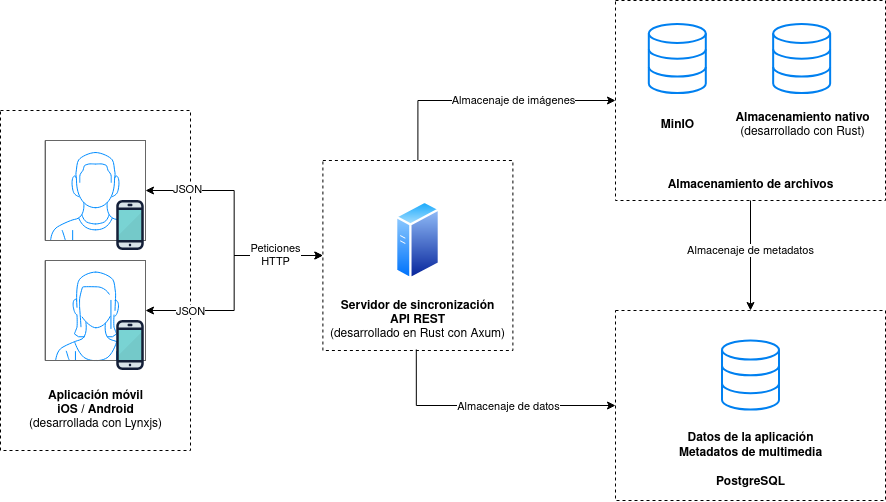
\includegraphics[width=0.95\textwidth]{images/diagrama-arquitectura.png}
    \end{center}
    \caption{Diagrama de la arquitectura del sistema. Representa las comunicaciones entre los distintos elementos del sistema}\label{fig:diagrama-arquitectura}
\end{figure}

Como podemos ver en la figura \ref{fig:diagrama-arquitectura}, el sistema va a estar compuesto por un cliente (móvil tanto en Android como iOS gracias a la multiplataforma que nos da Lynx.js) que se comunica con un servidor mediante peticiones HTTP.
Se estudió la posibilidad de la comunicación mediante gRPC (\textit{Google Remote Procedure Call}) pero se desechó ya que la compatibilidad entre un cliente multiplataforma desarrollado en Lynx.js (una tecnología muy nueva) y un servidor programado en Rust no permitía hacer uso de todas las ventajas que ofrecía frente a un método convencional como puede ser una API REST. Además, tanto Lynx.js como React Native no tienen muy buena compatibilidad con gRPC.

Todo esto hizo decidirse por una API REST, la cual es más sencilla de implementar y de mantener a largo plazo, además de ser más fácil de entender para cualquier desarrollador que quiera contribuir al proyecto.

El servidor se comunicará de manera abstracta con un servicio de almacenamiento de datos. Para la primera versión de la aplicación haremos uso de MinIO, un software Open-Source que nos permite crear un servidor de almacenamiento de objetos compatible con la API de Amazon S3.
Esto nos da la ventaja de poder utilizar cualquier servicio de almacenamiento compatible con S3 como Amazon S3, Google Cloud Storage en el futuro sin necesidad de cambiar la aplicación.
MinIO está diseñado para ser totalmente escalable y de alto rendimiento, lo que lo convierte en una excelente opción para almacenar grandes volúmenes de datos, como fotos y vídeos.

Aunque para las primeras iteraciones hagamos uso de MinIO para almacenar los datos multimedia, en iteraciones más avanzadas se implementará un sistema de almacenamiento nativo en Rust, el cual nos permitirá tener un mayor control sobre los datos y una mejor integración con el resto del sistema.

Gracias a la arquitectura hexagonal que se va a utilizar a la hora de implementar el sistema, conseguimos un desacople total de la capa de aplicación, dominio e infraestructura, brindando la posibilidad de cambiar la implementación de la capa de infraestructura sin afectar al resto del sistema, teniendo de esta manera flexibilidad sobre la solución que queramos usar para almacenar nuestros datos/multimedia.

Para el almacenaje de los datos de nuestra aplicación se ha optado por PostgreSQL.
Aunque puede ser menos escalable comparado con otras soluciones noSQL a largo plazo, nos da una gran cantidad de ventajas frente a las desventajas que tiene, como pueden ser:
\begin{itemize}
    \item \textbf{Integridad de los datos}: PostgreSQL es un sistema de gestión de bases de datos relacional, lo que significa que garantiza la integridad de los datos mediante el uso de transacciones y restricciones.
    \item \textbf{Escalabilidad}: aunque no es tan escalable como otras soluciones noSQL, PostgreSQL es capaz de manejar grandes volúmenes de datos y puede escalar horizontalmente mediante particionamiento.
    \item \textbf{Rendimiento}: PostgreSQL es conocido por su alto rendimiento y eficiencia en el manejo de consultas complejas y grandes volúmenes de datos.
    \item \textbf{Comunidad activa}: PostgreSQL tiene una comunidad muy activa y una gran cantidad de documentación y recursos disponibles, lo que facilita su aprendizaje y uso.
    \item \textbf{Open-Source}: al ser un software Open-Source, no tenemos que pagar por licencias y se alinea con el enfoque de nuestro proyecto que busca ser Open-Source.
\end{itemize}

\subsubsection{Estructura de implementación}
En un proyecto de este tipo es muy importante tener una buena estructura a la hora de implementar nuestras aplicaciones.
Buscamos la separación de responsabilidades y una buena organización lo cual nos lleva a cumplir uno de nuestros objetivos generales (OG4): desarrollar un sistema fácilmente escalable.

Para ello, se ha estudiado las distintas opciones que tenemos, tanto para el servidor como para la aplicación móvil, y principalmente se ha optado por una arquitectura limpia \parencite{uncle-bob-clean-architecture}, cuyos principios son:
\begin{itemize}
    \item \textbf{Separación de responsabilidades}: cada capa del sistema tiene una responsabilidad clara y bien definida, lo que facilita el mantenimiento y la evolución del sistema.
    \item \textbf{Independencia de la infraestructura}: las capas más internas del sistema no dependen de detalles de implementación de la infraestructura, lo que permite cambiar la infraestructura sin afectar al resto del sistema.
    \item \textbf{Facilidad de pruebas}: al tener una separación clara de responsabilidades, es más fácil realizar pruebas unitarias e integración, lo que mejora la calidad del software.
    \item \textbf{Escalabilidad}: al estar desacopladas las distintas capas del sistema, es más fácil escalar el sistema a medida que crece.
\end{itemize}

\paragraph{Arquitectura del servidor}
\subparagraph{}
Para el servidor se ha decidido usar una estructura monolítica modular siguiendo los principios de una arquitectura limpia.
Este enfoque se acerca a lo que sería una estructura de microservicios, pero sin la complejidad que conlleva el uso de múltiples servicios.
Siguiendo esta solución tenemos un solo binario que contiene todo el código del servidor, pero con una estructura modular, donde cada módulo tiene una responsabilidad clara y bien definida.
Es la mejor solución para un equipo pequeño por el simple hecho de que no tenemos que preocuparnos por la comunicación entre distintos servicios, el despliegue de los mismos y la gestión de la infraestructura para cada uno de los servicios.

Aún así, tenemos la gran mayoría de las ventajas que nos da una arquitectura de microservicios, como la separación de responsabilidades, la facilidad de pruebas y la escalabilidad.
De esta manera, si en un futuro quisiéramos separar el servidor en microservicios, sería mucho más sencillo hacerlo, ya que ya tenemos una estructura modular que nos permite separar las distintas funcionalidades del servidor.


\begin{figure}[H]
  \centering
  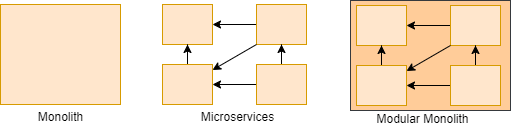
\includegraphics[width=0.8\textwidth]{assets/modular-monolith-comparison.png}
  \caption{Comparativa entre una arquitectura monolítica, de microservicios y monolítica modular. \parencite{tsechelidis2023modular}}
  \label{fig:modular-monolith-comparison}
\end{figure}

Como podemos ver en la figura \ref{fig:modular-monolith-comparison}, la diferencia que vemos entre una arquitectura de microservicios y una monolítica modular es que los módulos comparten el mismo proceso y por ende la comunicación entre ellos cambiará y se hará de manera local mediante llamadas a funciones, mientras que en una arquitectura de microservicios la comunicación entre los distintos servicios se hace mediante peticiones a través de un protocolo de comunicación específico y cada módulo tendría su propia forma de administrar datos, lo que añade una capa de complejidad innecesaria para un proyecto de este tipo.

\paragraph{Arquitectura del cliente}
\subparagraph{}
Tal y como se ha comentado anteriormente, la aplicación móvil también seguirá una arquitectura limpia, donde tendremos una capa de presentación, una capa de dominio y una capa de infraestructura.
La capa de presentación se encargará de la interfaz de usuario y de la interacción con el usuario, la capa de dominio se encargará de la lógica de negocio y la capa de infraestructura se encargará de la comunicación con el servidor y el almacenamiento local.

Tal como se comenta en el libro \textit{Clean Architecture} \parencite{uncle-bob-clean-architecture}, esta arquitectura es como una cebolla, donde cada capa está separada por una interfaz y cada capa puede comunicarse con la capa inferior a través de esta interfaz, pero no al revés.
Es decir, nuestra capa de dominio no se puede comunicar con ninguna de las otras capas, ya que esta es la capa más interna y no debe depender de ninguna otra capa.


\begin{figure}[H]
  \centering
  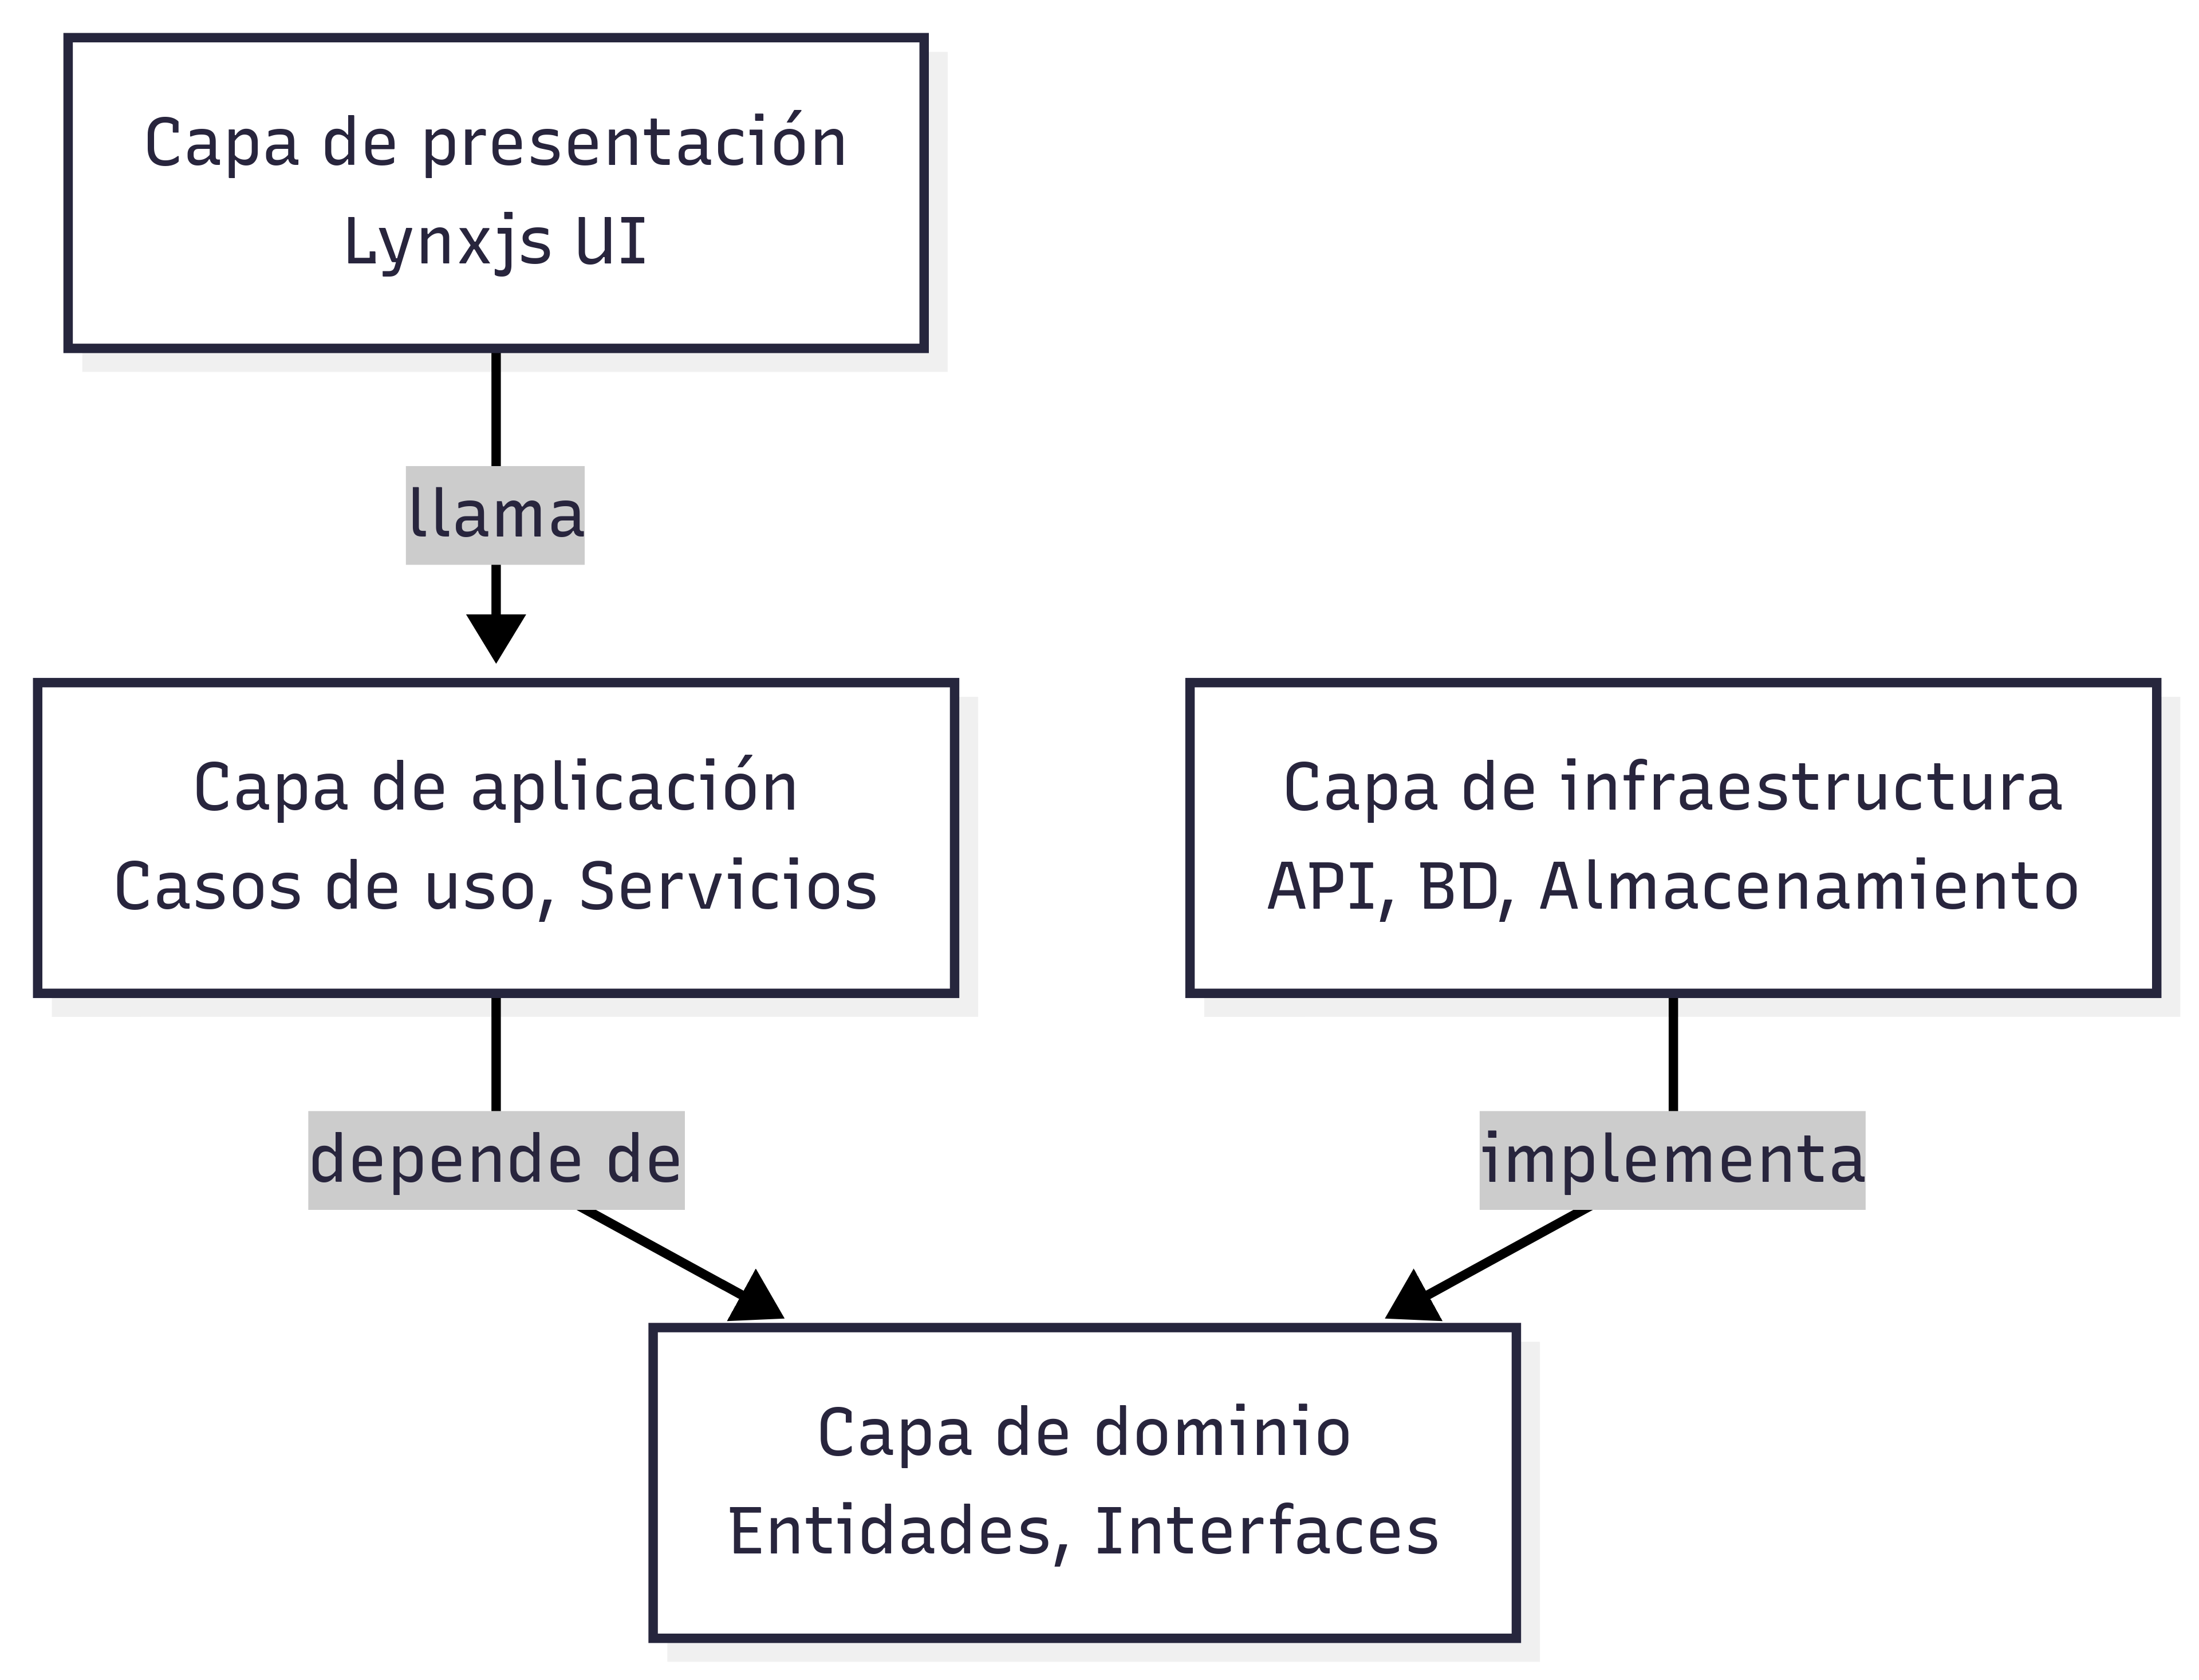
\includegraphics[width=0.8\textwidth]{assets/clean-architecture-mobile.png}
  \caption{Diagrama de arquitectura limpia en aplicación móvil.}
  \label{fig:clean-architecture-mobile}
\end{figure}

En la imagen podemos ver el diagrama de una arquitectura limpia para nuestra aplicación móvil, donde cada capa tiene una responsabilidad clara y bien definida.

Las flechas representan cómo accede cada capa a las demás.
El acceso se hace de la capa más externa a la más interna, es decir, la capa de dominio (la más interna) no puede saber nada sobre las otras capas, pero la capa de presentación puede acceder a la capa de dominio y a la capa de aplicación. 

Nuestra capa de aplicación no utiliza directamente la capa de infraestructura, sino que lo hace a través de interfaces que definimos en la capa de dominio. La capa de infraestructura se encarga de implementar estas interfaces, lo que nos permite cambiar la implementación de la capa de infraestructura sin afectar a la capa de dominio, de aplicación ni la de presentación.

De esta manera conseguimos una separación de responsabilidades y una independencia de la infraestructura, lo que nos permite cambiar la implementación de cualquier capa sin afectar al resto del sistema.
También nos permite hacer pruebas unitarias e integración de manera más sencilla, ya que podemos \gls{mockear} las interfaces de la capa de infraestructura y probar la lógica de negocio sin necesidad de depender de la implementación concreta de la capa de infraestructura.

\subsubsection{Inicialización del entorno de desarrollo}
En esta sección se va a detallar cómo se ha procedido a la inicialización del entorno de desarrollo tanto para el servidor como para la aplicación móvil.
\paragraph{Servidor}
\subparagraph{}
Para la inicialización del entorno de desarrollo del servidor nos hemos basado en la estructura de ejemplo que se puede encontrar en el artículo consultado sobre la arquitectura hexagonal en Rust \parencite{rust-hexagonal-architecture}. Éste quedaría de la siguiente manera:
\dirtree{%
.1 /.
.2 migrations/.
.3 20240603122606\_create\_authors.down.sql.
.3 20240603122606\_create\_authors.up.sql.
.2 src/.
.3 bin/.
.4 server/.
.5 main.rs.
.3 lib/.
.4 domain/.
.5 blog/.
.6 models/.
.7 author.rs.
.6 models.rs.
.6 ports.rs.
.6 service.rs.
.5 blog.rs.
.4 inbound/.
.5 http/.
.6 handlers/.
.7 create\_author.rs.
.6 handlers.rs.
.6 responses.rs.
.5 http.rs.
.4 outbound/.
.5 email\_client.rs.
.5 prometheus.rs.
.5 sqlite.rs.
.4 config.rs.
.4 domain.rs.
.4 inbound.rs.
.4 lib.rs.
.4 outbound.rs.
.2 .env.template.
.2 .gitignore.
.2 Cargo.lock.
.2 Cargo.toml.
.2 LICENSE.
.2 README.md.
}

Como podemos ver, tenemos la siguiente estructura:
\begin{itemize}
    \item \textbf{migrations}: esta carpeta contiene los archivos de migración de la base de datos, que se utilizan para crear y actualizar la estructura de la base de datos. En este caso, tenemos un archivo para crear la tabla de autores. Esta carpeta contiene todos los archivos necesarios para inicializar la base de datos y para borrarla si es necesario.
    \item \textbf{src}: esta carpeta contiene todo el código fuente del servidor, con las siguientes subcarpetas:
        \begin{itemize}
            \item \textbf{bin}: contiene el código que se ejecuta al iniciar el servidor, el punto de entrada de la aplicación. En esta carpeta no vamos a tener ningún tipo de lógica implementada, tan solo inicializaremos el servidor, definiremos las implementaciones de las interfaces y arrancaremos el servidor con las dependencias que necesite.
            \item \textbf{lib}: en esta carpeta tenemos todo el código de la aplicación, dividido siguiendo una filosofía hexagonal de la siguiente manera:
                \begin{itemize}
                    \item \textbf{domain}: contiene el código del dominio de la aplicación, es decir, la lógica de negocio. Aquí tenemos los modelos, definiciones de los puertos (interfaces) y servicios que se utilizan en la aplicación.
                    \item \textbf{inbound}: contiene el código de la capa de entrada de la aplicación, es decir, las interfaces que se exponen al exterior. En este caso, tenemos un módulo HTTP que define los handlers (controladores) que se encargan de recibir las peticiones HTTP y devolver las respuestas correspondientes.
                    \item \textbf{outbound}: contiene el código de la capa de salida de la aplicación, es decir, las implementaciones de las interfaces que se utilizan en la capa de dominio. En este caso, tenemos un cliente de correo electrónico, un cliente de Prometheus y un cliente SQLite que se encargan de enviar correos electrónicos, exponer métricas y acceder a la base de datos respectivamente.
                    \item \textbf{config.rs}: contiene la configuración de la aplicación, como las variables de entorno y los parámetros de configuración.
                    \item Los demás archivos definen los módulos de Rust.
                \end{itemize}
        \end{itemize}
\end{itemize}

Además de esos archivos, tenemos los archivos típicos de un proyecto de Rust, como son el \texttt{Cargo.toml} y el \texttt{Cargo.lock}, que definen las dependencias del proyecto y la versión de las mismas, así como el archivo \texttt{README.md} que contiene la documentación del proyecto y el archivo \texttt{LICENSE} que contiene la licencia del proyecto.

En nuestro proyecto, tal y como se ha definido anteriormente, vamos a utilizar un enfoque de arquitectura monolítica modular siguiendo el patrón de código \acrshort{cqrs}.
En este enfoque, los archivos van a estar organizados en módulos en vez de agrupados por capas, lo que nos va a permitir definir de una manera más clara y flexible las funcionalidades de cada módulo.
Además, en la capa de aplicación se separan los casos de uso en comandos y consultas (las consultas son las que se encargan de obtener datos y los comandos son los que se encargan de modificar el estado del sistema), lo que nos permite tener una mejor organización del código y una mayor flexibilidad a la hora de añadir nuevas funcionalidades.

Este es un enfoque común en aplicaciones web modernas, ya que gracias a esto podríamos conseguir funcionalidades como añadir caché a las consultas, realizar pruebas unitarias de los comandos y consultas de manera independiente, y tener una mejor organización del código en general.

Si adaptáramos este proyecto de ejemplo a la estructura que vamos a utilizar, tendríamos una estructura de la siguiente manera:

\newpage
\dirtree{%
.1 /.
.2 migrations/.
.3 20240603122606\_create\_authors.down.sql.
.3 20240603122606\_create\_authors.up.sql.
.2 src/.
.3 bin/.
.4 server/.
.5 main.rs.
.3 lib/.
.4 blog/.
.5 domain/.
.6 models.rs.
.6 models/.
.7 author.rs.
.6 ports.rs.
.5 application/.
.6 commands/.
.7 create\_author.rs.
.6 queries/.
.7 get\_authors.rs.
.5 infrastructure/.
.6 sqlite.rs.
.6 email\_client.rs.
.5 interface/.
.6 http/.
.7 handlers.rs.
.7 handlers/.
.8 create\_author.rs.
.7 responses.rs.
.4 monitoring/.
.5 infrastructure/.
.6 prometheus.rs.
.4 shared/.
.5 config.rs.
.5 lib.rs.
.2 .env.template.
.2 .gitignore.
.2 Cargo.lock.
.2 Cargo.toml.
.2 LICENSE.
.2 README.md.
}

\paragraph{Cliente móvil}
\subparagraph{}
Viendo la estructura del servidor y la definición de la arquitectura limpia para una aplicación móvil que hemos definido en la figura \ref{fig:clean-architecture-mobile}, podemos ver que la estructura del cliente móvil es muy similar a la del servidor, pero con algunas diferencias.

En este caso no vamos a utilizar el patrón de código \acrshort{cqrs}, ya que no es necesario en una aplicación móvil, pero sí vamos a utilizar una estructura modular similar a la del servidor, donde cada módulo tiene una responsabilidad clara y bien definida.
La única adición que tendremos con respecto a la estructura del servidor es que en la aplicación móvil tenemos una capa de presentación que se encarga de la interfaz de usuario y de la interacción con el usuario, la cual sería la equivalente a la capa de interface que definimos en el servidor para la comunicación con el exterior (en el caso del servidor, mediante comunicación HTTP).

Una estructura de ejemplo para una aplicación móvil que hace uso de el servidor de ejemplo que hemos definido anteriormente podría ser la siguiente:

\dirtree{%
.1 mobile-app/.
.2 src/.
.3 modules/.
.4 blog/.
.5 domain/.
.5 application/.
.6 services/.
.7 authorService.ts.
.7 blogService.ts.
.5 infrastructure/.
.5 presentation/.
.4 monitoring/.
.5 application/.
.6 services/.
.7 monitoringService.ts.
.5 infrastructure/.
.5 presentation/.
.4 shared/.
.5 config/.
.5 application/.
.6 services/.
.7 httpService.ts.
.7 storageService.ts.
.5 infrastructure/.
.5 presentation/.
.5 types/.
.3 navigation/.
.3 App.tsx.
.2 assets/.
.2 \_\_tests\_\_/.
.2 archivos de configuración del proyecto...
}

La principal diferencia que tenemos con respecto al servidor es que en la capa de aplicación no seguiremos un patrón CQRS y tendremos implementaciones de servicios que se encargan de toda la lógica.
Además, la capa de interfaz se cambia por una capa de presentación, que se encargará de la interfaz de usuario y de la interacción con el usuario.

Para la inicialización del entorno de desarrollo del cliente móvil, además del directorio que implementa nuestra aplicación usando Lynx.js necesitaremos un directorio para el código de Lynx Explorer, puesto que tendremos que hacer una implementación de módulos nativos para acceder a funcionalidades como el acceso a imágenes en el dispositivo tanto como para gestionar los permisos necesarios de la aplicación.
Toda la documentación que se ha utilizado para inicializar el directorio con nuestra versión de Lynx Explorer se puede encontrar en la \href{https://lynxjs.org/guide/use-native-modules.html#platform=android}{documentación oficial de Lynx.js} sobre implementación de módulos nativos.

\subsubsection{Desarrollo de artefactos del primer sprint}
Tal y como se ha definido en la \hyperref[sec:metodologia]{sección de metodología}, cada sprint se va a enfocar en una parte del proyecto. En este caso, el primer sprint se va a centrar en historias de usuario del servidor solamente. El segundo sprint se centrará en las historias de usuario del cliente móvil y una vez analizado el estado de ambos productos, se decidirá si comenzar a tener sprints conjuntos.

En la metodología Scrum se cogen historias de usuario hasta que la suma de las estimaciones de las historias de usuario sea menor o igual a la velocidad del equipo para ese sprint.
La velocidad del equipo se define como la cantidad de puntos de historia que el equipo puede completar en un sprint, y se calcula a partir de los sprints anteriores.
En este caso, como es el primer sprint y no tenemos una velocidad definida, se escogen historias de usuario fijándose en el tipo de tarea e intentando no tener una suma de puntos de historia muy alta.

Una vez se termina el sprint, en el proceso de retrospectiva se analiza cuántas historias de usuario se han completado o cuantas se han quedado a medias, y se ajusta la velocidad del equipo para el siguiente sprint. Este proceso se repite en cada sprint hasta que el equipo tiene una velocidad estable y podemos tener una estimación más precisa de cuántas historias de usuario se pueden completar en cada sprint.

Durante la especificación del sprint backlog se va a estudiar si hay historias de usuario que puedan ser divididas en distintas historias y una vez se hayan definido las historias de usuario que se van a implementar en el sprint, definiremos las tareas correspondientes a cada historia de usuario junto con su estimación en horas.
En el momento que tenemos estimaciones en horas de tareas, podemos realizar un diagrama de Gantt para el sprint con las tareas y su duración estimada.

\subsubsection{Planificación de entregas}
En esta sección se va a definir los objetivos generales que tendremos para cada entrega en caga sprint. Estos objetivos son estimados y pueden variar dependiendo de la velocidad real del equipo, puede ser que se consiga más en un sprint o menos. Esta planificación se realiza para que, en el caso de que tuviéramos un cliente, se le pudiera dar una estimación del producto que va a ir recibiendo en cada entrega.

En nuestro caso y en el tipo de proyecto que estamos realizando, nos sirve para tener un enfoque claro de lo que queremos conseguir en cada sprint y no desviarnos realizando otras tareas.
Definir qué se va a entregar en cada sprint nos ayuda también a priorizar qué historias de usuario se van a realizar en cada sprint.

Teniendo en cuenta que el desarrollo del proyecto comienza la última semana de junio de 2025, que cada sprint dura dos semanas y que la fecha límite de entrega del proyecto es el 5 de septiembre de 2025, tenemos un total de 11 semanas para el proyecto. Teniendo en cuenta que el sprint 0 tiene una duración de una semana, tenemos un total de 5 sprints para el desarrollo del proyecto.

Los objetivos de cada sprint quedarían de la siguiente manera:
\begin{itemize}
    \item \textbf{Sprint 1}: Implementación de la API REST del servidor, incluyendo la gestión de usuarios, autenticación y autorización, así como la subida y descarga de archivos. Durante esta iteración se busca implementar una subida y descarga de archivos básica y genérica.
    \item \textbf{Sprint 2}: Implementación de la aplicación móvil. Definición e implementación de módulos nativos para el acceso a archivos multimedia y permisos. Durante esta iteración se busca implementar una aplicación de gestión de galería básica sin funcionalidades de sincronización. 
    \item \textbf{Sprint 3}: Implementación de todo el procesado multimedia en el servidor: generación de miniaturas, compresión de imágenes y vídeos, etiquetado basado en metadatos, etc. En el cliente se implementará la subida de archivos multimedia a el servidor y la visualización de los archivos subidos.
    \item \textbf{Sprint 4}: Implementación de la sincronización automática de archivos multimedia en el cliente móvil tanto como la visualización del estado nuestra galería en el servidor. En esta iteración implementaremos principalmente toda la conexión automática entre el cliente y el servidor, así como la sincronización de archivos multimedia.
    \item \textbf{Sprint 5}: Implementación de la gestión de usuarios desde el cliente móvil, incluyendo la gestión de permisos en las galerías, álbumes y archivos. Durante esta última iteración se implementará el uso compartido de galerías y álbumes entre usuarios.
    \item \textbf{Sprint 6}: Implementación de interfaz de usuario para gestión de configuración del servidor. Implementación de servicio de almacenamiento de archivos multimedia propio en el servidor. Éste último sprint, aunque no entra en el plazo de entrega del proyecto, se define para tener una idea de lo que se quiere conseguir en el futuro, poder tener una planificación más clara de lo que se quiere conseguir en el proyecto y facilitar contribuciones al proyecto open-source.
\end{itemize}

Tal y como se ha mencionado anteriormente, estos objetivos son estimados y por la naturaleza de la metodología Scrum pueden ir variando a lo largo del desarrollo. Al final de cada sprint se realizará una retrospectiva donde se ajustarán los backlogs y objetivos de los siguientes sprints en función de lo que se haya conseguido en el sprint anterior.

\subsection{Presupuesto}
\label{sec:presupuesto}
Para el cálculo y desglose del presupuesto total del proyecto se ha supuesto un equipo de una única persona a media jornada.

Para el cálculo del presupuesto de personal hemos tenido en cuenta el salario medio de un ingeniero de software en España, que según el portal de empleo \href{https://www.glassdoor.es/Sueldos/granada-software-engineer-sueldo-SRCH_IL.0,7_IC2614045_KO8,25.htm}{Glassdoor} ronda entre los 24.000 y 33.000 euros brutos anuales, cogiendo el valor de 24000 euros brutos anuales como salario base dada la inexperiencia del trabajador.

Para calcular el costo total mensual de un trabajador, tenemos que sumar a el salario base los costes de seguridad social, la cuota patronal y el \acrshort{irpf}, siguiendo la siguiente fórmula:
\begin{equation}
    \text{Coste total mensual} = \text{Salario base} + \text{Seguridad Social} + \text{Cuota patronal} + \text{IRPF}
\end{equation}
\begin{itemize}
    \item Salario base: 12.000 euros brutos anuales / 12 meses = 1.000 euros brutos mensuales
    \item Seguridad social: se entiende por seguridad social a la cuota obrera que debe de pagar el trabajador. En este caso se debe aplicar el 6.45\% sobre el salario bruto mensual. Por lo tanto:
        \begin{equation}
            \text{Seguridad Social} = 1000 \times 0.0645 = 64.5 \text{ euros mensuales}
        \end{equation}
    \item Cuota patronal: se entiende por cuota patronal a la cuota que debe de pagar la empresa por el trabajador.
        Según la base mínima de cotización para 2024 de un ingeniero técnico (1.532,10 euros\footnote{Fuente: \href{https://www.cuestioneslaborales.es/porcentaje-de-cotizacion-a-la-seguridad-social-del-trabajador-y-empresa/}{Porcentaje de cotización a la Seguridad Social del trabajador y empresa} entre 2 ya que es media jornada\textit{ Última vez accedido el 20/06/2025 }}) se ha aplicado el porcentaje de cotización del 31,98\%.
        Nuestro cálculo es el siguiente:
        \begin{equation}
            \text{Cuota patronal} = \dfrac{1532.10 \times 0.3198}{2} = 245.12 \text{ euros mensuales}
        \end{equation}
    \item IRPF: con un salario bruto anual de 12.000 euros, en 2024 el IRPF que aplica es del 19\% \footnote{Fuente: \href{https://www.bankinter.com/blog/finanzas-personales/como-calcular-retenciones-irpf-nomina\#tabla-retenciones}{Cómo calcular retenciones IRPF en la nómina}\textit{ Última vez accedido el 20/06/2025 }}.
        Por lo tanto, el IRPF mensual sería:
        \begin{equation}
            \text{IRPF} = 1000 \times 0.19 = 190 \text{ euros mensuales}
        \end{equation}
\end{itemize}

De esta manera, el coste total mensual del trabajador sería:
\begin{equation}
    \text{Coste total mensual} = 1000 + 64.5 + 245.12 + 190 = 1499.62 \text{ euros mensuales}
\end{equation}

Para el gasto de materiales solamente tendremos materiales inventables, concretamente el material de trabajo del trabajador.
Dicho material de trabajo sería el siguiente:
\begin{itemize}
    \item Ordenador de sobremesa: 1.000 euros con vida estimada restante de 4 años, es decir, 250 euros al año.
    \item Monitores: 300 euros con vida estimada restante de 6 años, es decir, 50 euros al año.
    \item Teclado y ratón: 150 euros con vida estimada restante de 3 años, es decir, 50 euros al año.
\end{itemize}
La duración total del proyecto es de 3 meses, por lo que el coste total de materiales sería:
\begin{equation}
    \text{Coste total de materiales} = \dfrac{250 + 50 + 50}{12} \times 3 = 37.5 \text{ euros}
\end{equation}

Dado que uno de los objetivos principales del proyecto es la capacidad de alojar la aplicación en un servidor propio, no tenemos en cuenta el coste de un servidor.

Dado que la aplicación se ha desarrollado usando Rust y Lynx.js, no se han tenido en cuenta los costes de licencias de software, ya que ambas tecnologías son Open-Source y no requieren de licencias para su uso.

Para la formación del trabajador se han usado cursos gratuitos así como la documentación oficial de las tecnologías utilizadas, por lo que no se ha tenido en cuenta ningún coste adicional.

De esta forma, tendríamos el siguiente desglose de costes:
\begin{table}[H]
    \caption{Tabla de presupuesto del proyecto}\label{tab:presupuesto}
    \begin{center}
        \begin{tabularx}{\textwidth}{|X|c|c|c|}
            \hline
            \textbf{Gastos elegibles} & \textbf{Unidades} & \textbf{Coste por unidad} & \textbf{Importe solicitado} \\
            \hline
            \multicolumn{3}{|l|}{\textbf{GASTOS DE PERSONAL}} & \textbf{4.498.86\euro} \\
            Total gastos de contratación de personal & 3 & 1.499,62\euro/mes & 4.498,86\euro \\
            \hline
            \multicolumn{3}{|l|}{\textbf{GASTOS DE EJECUCIÓN}} & \textbf{87.5\euro} \\
            \multicolumn{3}{|l|}{Costes de adquisición de material inventariable} & 87.5\euro \\
            \quad Ordenador & 1 & 62,50\euro & 62,50\euro \\
            \quad Monitores & 1 & 12,50\euro & 12,50\euro \\
            \quad Teclado y ratón & 1 & 12,50\euro & 12,50\euro \\
            \multicolumn{3}{|l|}{Costes de adquisición de material fungible} & 0\euro \\
            \multicolumn{3}{|l|}{Costes de consultoría, prestación de servicios, suministros, etc.} & 0\euro \\
            \multicolumn{3}{|l|}{Costes de subcontratación} & 0\euro \\
            \multicolumn{3}{|l|}{\textbf{GASTOS COMPLEMENTARIOS}} & \textbf{0\euro} \\
            \multicolumn{3}{|l|}{Formación del equipo de desarrollo} & 0\euro \\
            \multicolumn{3}{|l|}{Gastos de desplazamiento, viajes, estancias y dietas} & 0\euro \\
            \multicolumn{3}{|l|}{Gastos de inscripción en congresos y seminarios} & 0\euro \\
            \hline
            \multicolumn{3}{|l|}{\textbf{COSTES DIRECTOS (10\% presupuesto total)}} & \textbf{458,64\euro} \\
            \hline
            \multicolumn{3}{|l|}{\textbf{TOTAL INCENTIVO SOLICITADO}} & \textbf{5.045,00\euro} \\
            \hline
        \end{tabularx}
    \end{center}
\end{table}

\section{Sprint 1}
Tal y como se ha definido en la sección \ref{sec:planificacion-inicial}, el primer sprint se centra en la base de nuestra aplicación web, desarrollando la estructura inicial del servidor, gestión de usuarios y subida y descarga sencilla de archivos.
Para ello, se han elegido las historias de usuario relacionadas con el objetivo de este sprint y se han desarrollado definiendo sub-historias de usuario si fueran necesarias, criterios de aceptación y las tareas necesarias para su implementación.

Las historias de usuario se han seleccionado de manera aproximada, puesto que al ser el primer sprint no tenemos una velocidad de equipo definida. Existe la posibilidad de que algunas historias de usuario no se completen en este sprint o de que se completen más de las previstas, por lo que se ha dejado un margen de maniobra para que el equipo pueda adaptarse a la realidad del desarrollo.

Cuando se termine el sprint, se calculará la velocidad del equipo la cual se utilizará para planificar los siguientes sprints, de manera que se pueda ajustar la cantidad de historias de usuario a desarrollar en cada uno de ellos.

Una vez definidas todas las tareas que se van a realizar en este sprint, se ha realizado un diagrama de Gantt para planificar el tiempo que se va a dedicar a cada una de ellas, teniendo en cuenta que el sprint tiene una duración de dos semanas, y se dará un orden de prioridad a las tareas que se consideren más importantes para llegar a el objetivo del sprint.

\subsection{Historias de usuario}
En esta sección se detallan las historias de usuario y técnicas que se han elegido para este sprint. Se va a hacer una breve descripción de cada una de ellas, así como los criterios de aceptación y las tareas necesarias para su implementación. Si fuera necesario, se definirán sub-historias de usuario para facilitar su desarrollo.

Las seleccionadas son las siguientes:
\begin{itemize}
    \item HU05: Inicio de sesión - 5 PH
    \item HU06: Cerrar sesión - 2 PH
    \item HU13: Crear cuentas - 8 PH
    \item HT03 API REST en Rust - 13 PH
    \item HT05: Autenticación JWT - 5 PH
    \item HT08: Base de datos - 8 PH
    \item HT18.1: Binario - 2 PH
    \item HT19: Dockerización - 3 PH
    \item HT20.1: Documentación del proyecto en GitHub - 5 PH
    \item HT20.2: Documentación de la API REST con OpenAPI - 5 PH
\end{itemize}

Estas historias de usuario y técnicas suman un total de 56 puntos de historia (PH). Es importante destacar que la estimación en puntos de historia representa la complejidad relativa de cada historia, mientras que las tareas de desarrollo se estiman en horas de trabajo efectivo.

\paragraph{Descomposición en tareas de desarrollo}

% HU05: Inicio de sesión
\begin{table}[H]
    \begin{center}
        \begin{tabularx}{\textwidth}{|l|X|l|}
            \hline
            \textbf{Identificador HU05} & 
            \textbf{Como usuario, quiero iniciar sesión con contraseña o clave, para evitar que otros accedan a mis archivos} &
            \textbf{Estimación: 5 PH}\\
            \hline
            \multicolumn{3}{|p{\textwidth}|}{
                \begin{minipage}{\textwidth}
                    \centering
                    \vspace{0.5em}
                    \begin{tabular}{|l|p{8cm}|r|}
                        \hline
                        \textbf{Identificador} & \textbf{Título de la tarea de desarrollo} & \makecell{\textbf{Estimación}\\\textbf{(h)}} \\
                        \hline
                        Tarea 5-1 & Implementar endpoint para iniciar sesión & 2 \\
                        \hline
                        Tarea 5-2 & Validar credenciales de usuario contra la base de datos & 1.5 \\
                        \hline
                        Tarea 5-3 & Generar y devolver token JWT al usuario autenticado & 1.5 \\
                        \hline
                        Tarea 5-4 & Gestionar errores de autenticación (usuario no existe, contraseña incorrecta) & 1.5 \\
                        \hline
                        Tarea 5-5 & Documentar el endpoint de inicio de sesión en OpenAPI & 0.5 \\
                        \hline
                    \end{tabular}
                    \vspace{0.5em}
                \end{minipage}
            } \\
            \hline
            \multicolumn{3}{|p{\textwidth}|}{
                \textbf{Pruebas de aceptación:}
                    \begin{itemize}
                        \item El usuario puede iniciar sesión con su contraseña.
                        \item Cuando el usuario inicia sesión, se le devuelve un token JWT.
                        \item Si el usuario no existe, se devuelve un mensaje de error.
                        \item Si la contraseña o clave son incorrectas, se devuelve un mensaje de error.
                        \item El endpoint está documentado en OpenAPI.
                    \end{itemize}
            }\\
            \hline
            \multicolumn{3}{|p{\textwidth}|}{
                \textbf{Observaciones:}
                \begin{itemize}
                    \item El endpoint debe ser seguro (usar HTTPS).
                    \item El token JWT debe tener expiración configurable.
                \end{itemize}
            }\\
            \hline
        \end{tabularx}
    \end{center}
\end{table}

% HU06: Cerrar sesión
\begin{table}[H]
    \begin{center}
        \begin{tabularx}{\textwidth}{|l|X|l|}
            \hline
            \textbf{Identificador HU06} & 
            \textbf{Como usuario, quiero poder cerrar sesión en un dispositivo, para proteger mis datos si pierdo el móvil} &
            \textbf{Estimación: 2 PH}\\
            \hline
            \multicolumn{3}{|c|}{
                \begin{minipage}{\linewidth}
                    \centering
                    \vspace{0.5em}
                    \begin{tabular}{|l|p{8cm}|r|}
                        \hline
                        \textbf{Identificador} & \textbf{Título de la tarea de desarrollo} & \makecell{\textbf{Estimación}\\\textbf{(h)}} \\
                        \hline
                        Tarea 6-1 & Implementar endpoint para cerrar sesión (invalidar token JWT) & 1 \\
                        \hline
                        Tarea 6-2 & Gestionar lista negra de tokens JWT (opcional) & 1 \\
                        \hline
                    \end{tabular}
                    \vspace{0.5em}
                \end{minipage}
            } \\
            \hline
            \multicolumn{3}{|p{\textwidth}|}{
                \textbf{Pruebas de aceptación:}
                    \begin{itemize}
                        \item El usuario puede cerrar sesión y su token queda invalidado.
                        \item Tras cerrar sesión, el token no permite acceder a endpoints protegidos.
                    \end{itemize}
            }\\
            \hline
            \multicolumn{3}{|p{\textwidth}|}{
                \textbf{Observaciones:}
                \begin{itemize}
                    \item Si no se implementa lista negra, el token expira por tiempo.
                \end{itemize}
            }\\
            \hline
        \end{tabularx}
    \end{center}
\end{table}

% HU13: Crear cuentas
\begin{table}[H]
    \begin{center}
        \begin{tabularx}{\textwidth}{|l|X|l|}
            \hline
            \textbf{Identificador HU13} & 
            \textbf{Como administrador, quiero crear cuentas de usuario con permisos, para que varias personas puedan usar el servidor} &
            \textbf{Estimación: 8 PH}\\
            \hline
            \multicolumn{3}{|c|}{
                \begin{minipage}{\linewidth}
                    \centering
                    \vspace{0.5em}
                    \begin{tabular}{|l|p{8cm}|r|}
                        \hline
                        \textbf{Identificador} & \textbf{Título de la tarea de desarrollo} & \makecell{\textbf{Estimación}\\\textbf{(h)}} \\
                        \hline
                        Tarea 13-1 & Implementar endpoint para crear cuentas de usuario & 2 \\
                        \hline
                        Tarea 13-2 & Validar permisos de administrador para crear cuentas & 1.5 \\
                        \hline
                        Tarea 13-3 & Añadir roles/permisos a los usuarios & 1.5 \\
                        \hline
                        Tarea 13-4 & Gestionar almacenamiento seguro de contraseñas (hash) & 1.5 \\
                        \hline
                        Tarea 13-5 & Documentar el endpoint de creación de cuentas en OpenAPI & 0.5 \\
                        \hline
                        Tarea 13-6 & Pruebas unitarias de creación de usuario & 1 \\
                        \hline
                    \end{tabular}
                    \vspace{0.5em}
                \end{minipage}
            } \\
            \hline
            \multicolumn{3}{|p{\textwidth}|}{
                \textbf{Pruebas de aceptación:}
                    \begin{itemize}
                        \item Solo el administrador puede crear cuentas.
                        \item El usuario creado puede iniciar sesión.
                        \item Los roles/permisos se asignan correctamente.
                        \item El endpoint está documentado en OpenAPI.
                    \end{itemize}
            }\\
            \hline
            \multicolumn{3}{|p{\textwidth}|}{
                \textbf{Observaciones:}
                \begin{itemize}
                    \item Usar hash seguro para contraseñas (ej: Argon2).
                \end{itemize}
            }\\
            \hline
        \end{tabularx}
    \end{center}
\end{table}

% HT03: API REST en Rust
\begin{table}[H]
    \begin{center}
        \begin{tabularx}{\textwidth}{|l|X|l|}
            \hline
            \textbf{Identificador HT03} & 
            \textbf{Desarrollar API RESTful usando Rust y Axum} &
            \textbf{Estimación: 13 PH}\\
            \hline
            \multicolumn{3}{|c|}{
                \begin{minipage}{\linewidth}
                    \centering
                    \vspace{0.5em}
                    \begin{tabular}{|l|p{8cm}|r|}
                        \hline
                        \textbf{Identificador} & \textbf{Título de la tarea de desarrollo} & \makecell{\textbf{Estimación}\\\textbf{(h)}} \\
                        \hline
                        Tarea 3-1 & Crear estructura base del proyecto en Rust & 2 \\
                        \hline
                        Tarea 3-2 & Configurar Axum y dependencias principales & 2 \\
                        \hline
                        Tarea 3-3 & Definir rutas y controladores básicos & 2 \\
                        \hline
                        Tarea 3-4 & Implementar manejo de errores global & 2 \\
                        \hline
                        Tarea 3-5 & Añadir middlewares (logging, CORS, etc.) & 1.5 \\
                        \hline
                        Tarea 3-6 & Configurar variables de entorno y settings & 1.5 \\
                        \hline
                        Tarea 3-7 & Documentar endpoints iniciales & 1 \\
                        \hline
                        Tarea 3-8 & Pruebas de integración básicas & 1 \\
                        \hline
                    \end{tabular}
                    \vspace{0.5em}
                \end{minipage}
            } \\
            \hline
            \multicolumn{3}{|p{\textwidth}|}{
                \textbf{Pruebas de aceptación:}
                    \begin{itemize}
                        \item El servidor arranca y responde a peticiones básicas.
                        \item Los endpoints definidos funcionan correctamente.
                        \item El manejo de errores es consistente.
                    \end{itemize}
            }\\
            \hline
            \multicolumn{3}{|p{\textwidth}|}{
                \textbf{Observaciones:}
                \begin{itemize}
                    \item Seguir estructura modular y buenas prácticas de Rust.
                \end{itemize}
            }\\
            \hline
        \end{tabularx}
    \end{center}
\end{table}

% HT05: Autenticación JWT
\begin{table}[H]
    \begin{center}
        \begin{tabularx}{\textwidth}{|l|X|l|}
            \hline
            \textbf{Identificador HT05} & 
            \textbf{Implementar autenticación con JSON Web Tokens} &
            \textbf{Estimación: 5 PH}\\
            \hline
            \multicolumn{3}{|c|}{
                \begin{minipage}{\linewidth}
                    \centering
                    \vspace{0.5em}
                    \begin{tabular}{|l|p{8cm}|r|}
                        \hline
                        \textbf{Identificador} & \textbf{Título de la tarea de desarrollo} & \makecell{\textbf{Estimación}\\\textbf{(h)}} \\
                        \hline
                        Tarea 5-1 & Añadir librería de JWT y configuración & 1.5 \\
                        \hline
                        Tarea 5-2 & Implementar generación y validación de tokens & 1.5 \\
                        \hline
                        Tarea 5-3 & Proteger endpoints con autenticación JWT & 1 \\
                        \hline
                        Tarea 5-4 & Pruebas unitarias de autenticación & 1 \\
                        \hline
                    \end{tabular}
                    \vspace{0.5em}
                \end{minipage}
            } \\
            \hline
            \multicolumn{3}{|p{\textwidth}|}{
                \textbf{Pruebas de aceptación:}
                    \begin{itemize}
                        \item Solo usuarios autenticados pueden acceder a endpoints protegidos.
                        \item Los tokens inválidos o expirados son rechazados.
                    \end{itemize}
            }\\
            \hline
            \multicolumn{3}{|p{\textwidth}|}{
                \textbf{Observaciones:}
                \begin{itemize}
                    \item Usar claves seguras y expiración adecuada.
                \end{itemize}
            }\\
            \hline
        \end{tabularx}
    \end{center}
\end{table}

% HT08: Base de datos
\begin{table}[H]
    \begin{center}
        \begin{tabularx}{\textwidth}{|l|X|l|}
            \hline
            \textbf{Identificador HT08} & 
            \textbf{Implementar SQLite o PostgreSQL para usuarios y archivos} &
            \textbf{Estimación: 8 PH}\\
            \hline
            \multicolumn{3}{|c|}{
                \begin{minipage}{\linewidth}
                    \centering
                    \vspace{0.5em}
                    \begin{tabular}{|l|p{8cm}|r|}
                        \hline
                        \textbf{Identificador} & \textbf{Título de la tarea de desarrollo} & \makecell{\textbf{Estimación}\\\textbf{(h)}} \\
                        \hline
                        Tarea 8-1 & Definir modelo de datos para usuarios y archivos & 2 \\
                        \hline
                        Tarea 8-2 & Crear migraciones iniciales de la base de datos & 1.5 \\
                        \hline
                        Tarea 8-3 & Implementar acceso a base de datos en Rust & 2 \\
                        \hline
                        Tarea 8-4 & Pruebas de persistencia y consultas básicas & 1.5 \\
                        \hline
                    \end{tabular}
                    \vspace{0.5em}
                \end{minipage}
            } \\
            \hline
            \multicolumn{3}{|p{\textwidth}|}{
                \textbf{Pruebas de aceptación:}
                    \begin{itemize}
                        \item Se pueden crear, consultar y modificar usuarios y archivos.
                        \item Las migraciones funcionan correctamente.
                    \end{itemize}
            }\\
            \hline
            \multicolumn{3}{|p{\textwidth}|}{
                \textbf{Observaciones:}
                \begin{itemize}
                    \item Usar ORM recomendado para Rust (ej: sqlx, diesel).
                \end{itemize}
            }\\
            \hline
        \end{tabularx}
    \end{center}
\end{table}

% HT18.1: Binario
\begin{table}[H]
    \begin{center}
        \begin{tabularx}{\textwidth}{|l|X|l|}
            \hline
            \textbf{Identificador HT18.1} & 
            \textbf{Empaquetar la aplicación como un solo binario} &
            \textbf{Estimación: 2 PH}\\
            \hline
            \multicolumn{3}{|c|}{
                \begin{minipage}{\linewidth}
                    \centering
                    \vspace{0.5em}
                    \begin{tabular}{|l|p{8cm}|r|}
                        \hline
                        \textbf{Identificador} & \textbf{Título de la tarea de desarrollo} & \makecell{\textbf{Estimación}\\\textbf{(h)}} \\
                        \hline
                        Tarea 18.1-1 & Configurar build para generar binario único & 1.5 \\
                        \hline
                        Tarea 18.1-2 & Verificar funcionamiento del binario en distintos entornos & 0.5 \\
                        \hline
                    \end{tabular}
                    \vspace{0.5em}
                \end{minipage}
            } \\
            \hline
            \multicolumn{3}{|p{\textwidth}|}{
                \textbf{Pruebas de aceptación:}
                    \begin{itemize}
                        \item El binario se genera correctamente y es ejecutable.
                        \item El binario funciona en los sistemas operativos objetivo.
                    \end{itemize}
            }\\
            \hline
            \multicolumn{3}{|p{\textwidth}|}{
                \textbf{Observaciones:}
                \begin{itemize}
                    \item Documentar el proceso de build en el README.
                \end{itemize}
            }\\
            \hline
        \end{tabularx}
    \end{center}
\end{table}

% HT19: Dockerización
\begin{table}[H]
    \begin{center}
        \begin{tabularx}{\textwidth}{|l|X|l|}
            \hline
            \textbf{Identificador HT19} & 
            \textbf{Crear imagen Docker del servidor} &
            \textbf{Estimación: 3 PH}\\
            \hline
            \multicolumn{3}{|c|}{
                \begin{minipage}{\linewidth}
                    \centering
                    \vspace{0.5em}
                    \begin{tabular}{|l|p{8cm}|r|}
                        \hline
                        \textbf{Identificador} & \textbf{Título de la tarea de desarrollo} & \makecell{\textbf{Estimación}\\\textbf{(h)}} \\
                        \hline
                        Tarea 19-1 & Crear Dockerfile para el servidor & 1.5 \\
                        \hline
                        Tarea 19-2 & Configurar variables de entorno y volúmenes & 1 \\
                        \hline
                        Tarea 19-3 & Probar despliegue local y documentar uso & 0.5 \\
                        \hline
                    \end{tabular}
                    \vspace{0.5em}
                \end{minipage}
            } \\
            \hline
            \multicolumn{3}{|p{\textwidth}|}{
                \textbf{Pruebas de aceptación:}
                    \begin{itemize}
                        \item El servidor se ejecuta correctamente en un contenedor Docker.
                        \item Se pueden configurar variables y volúmenes.
                    \end{itemize}
            }\\
            \hline
            \multicolumn{3}{|p{\textwidth}|}{
                \textbf{Observaciones:}
                \begin{itemize}
                    \item Seguir buenas prácticas de Docker (multi-stage build si es posible).
                \end{itemize}
            }\\
            \hline
        \end{tabularx}
    \end{center}
\end{table}

% HT20.1: Documentación del proyecto en GitHub
\begin{table}[H]
    \begin{center}
        \begin{tabularx}{\textwidth}{|l|X|l|}
            \hline
            \textbf{Identificador HT20.1} & 
            \textbf{Documentar la instalación y uso del proyecto en el repositorio de Github} &
            \textbf{Estimación: 5 PH}\\
            \hline
            \multicolumn{3}{|c|}{
                \begin{minipage}{\linewidth}
                    \centering
                    \vspace{0.5em}
                    \begin{tabular}{|l|p{8cm}|r|}
                        \hline
                        \textbf{Identificador} & \textbf{Título de la tarea de desarrollo} & \makecell{\textbf{Estimación}\\\textbf{(h)}} \\
                        \hline
                        Tarea 20.1-1 & Redactar README con instrucciones de instalación & 1 \\
                        \hline
                        Tarea 20.1-2 & Documentar configuración y variables de entorno & 1 \\
                        \hline
                        Tarea 20.1-3 & Añadir ejemplos de uso y comandos básicos & 1 \\
                        \hline
                        Tarea 20.1-4 & Revisar y mejorar formato y claridad & 1 \\
                        \hline
                    \end{tabular}
                    \vspace{0.5em}
                \end{minipage}
            } \\
            \hline
            \multicolumn{3}{|p{\textwidth}|}{
                \textbf{Pruebas de aceptación:}
                    \begin{itemize}
                        \item El README permite instalar y ejecutar el proyecto desde cero.
                        \item Toda la configuración necesaria está documentada.
                    \end{itemize}
            }\\
            \hline
            \multicolumn{3}{|p{\textwidth}|}{
                \textbf{Observaciones:}
                \begin{itemize}
                    \item Usar ejemplos claros y comandos reproducibles.
                \end{itemize}
            }\\
            \hline
        \end{tabularx}
    \end{center}
\end{table}

% HT20.2: Documentación de la API REST con OpenAPI
\begin{table}[H]
    \begin{center}
        \begin{tabularx}{\textwidth}{|l|X|l|}
            \hline
            \textbf{Identificador HT20.2} & 
            \textbf{Documentar mediante la generación de una página web todos los endpoints de la API REST} &
            \textbf{Estimación: 5 PH}\\
            \hline
            \multicolumn{3}{|c|}{
                \begin{minipage}{\linewidth}
                    \centering
                    \vspace{0.5em}
                    \begin{tabular}{|l|p{8cm}|r|}
                        \hline
                        \textbf{Identificador} & \textbf{Título de la tarea de desarrollo} & \makecell{\textbf{Estimación}\\\textbf{(h)}} \\
                        \hline
                        Tarea 20.2-1 & Generar especificación OpenAPI de la API REST & 1.5 \\
                        \hline
                        Tarea 20.2-2 & Añadir descripciones y ejemplos a los endpoints & 1.5 \\
                        \hline
                        Tarea 20.2-3 & Publicar documentación como página web (Swagger UI u OpenAPI UI) & 1 \\
                        \hline
                        Tarea 20.2-4 & Revisar y mantener la documentación actualizada & 1 \\
                        \hline
                    \end{tabular}
                    \vspace{0.5em}
                \end{minipage}
            } \\
            \hline
            \multicolumn{3}{|p{\textwidth}|}{
                \textbf{Pruebas de aceptación:}
                    \begin{itemize}
                        \item Todos los endpoints están documentados y accesibles vía web.
                        \item La documentación incluye ejemplos de peticiones y respuestas, tanto respuestas exitosas como errores.
                        \item La documentación se actualiza automáticamente al cambiar el código.
                    \end{itemize}
            }\\
            \hline
            \multicolumn{3}{|p{\textwidth}|}{
                \textbf{Observaciones:}
                \begin{itemize}
                    \item Usar herramientas automáticas para mantener la documentación sincronizada.
                \end{itemize}
            }\\
            \hline
        \end{tabularx}
    \end{center}
\end{table}

\paragraph{Resumen de estimación de tareas}

El total de horas estimadas para todas las tareas de desarrollo del Sprint 1 es de 56 horas, distribuidas de la siguiente manera:

\begin{itemize}
    \item HU05 (Inicio de sesión): 7 horas
    \item HU06 (Cerrar sesión): 2 horas  
    \item HU13 (Crear cuentas): 8 horas
    \item HT03 (API REST en Rust): 13 horas
    \item HT05 (Autenticación JWT): 5 horas
    \item HT08 (Base de datos): 7 horas
    \item HT18.1 (Binario): 2 horas
    \item HT19 (Dockerización): 3 horas
    \item HT20.1 (Documentación GitHub): 4 horas
    \item HT20.2 (Documentación OpenAPI): 5 horas
\end{itemize}

Esta estimación se ajusta perfectamente a la capacidad del sprint de 2 semanas con 4 horas diarias de dedicación (14 días × 4 horas = 56 horas totales).

Se puede ver que hay historias de usuario con los mismos puntos de historia o parecidos pero con diferente número de horas estimadas. Esto es normal, ya que los puntos de historia representan la complejidad relativa y no el tiempo exacto de desarrollo. Por ejemplo, una historia de usuario puede ser más compleja pero requerir menos tiempo si se reutilizan componentes existentes o se aprovechan bibliotecas ya implementadas.

\subsection{Diagrama de Gantt}
Dada las estimaciones de las tareas, se han considerado el siguiente orden de prioridad de tareas en un diagrama de Gantt:
\begin{figure}[H]
    \begin{center}
        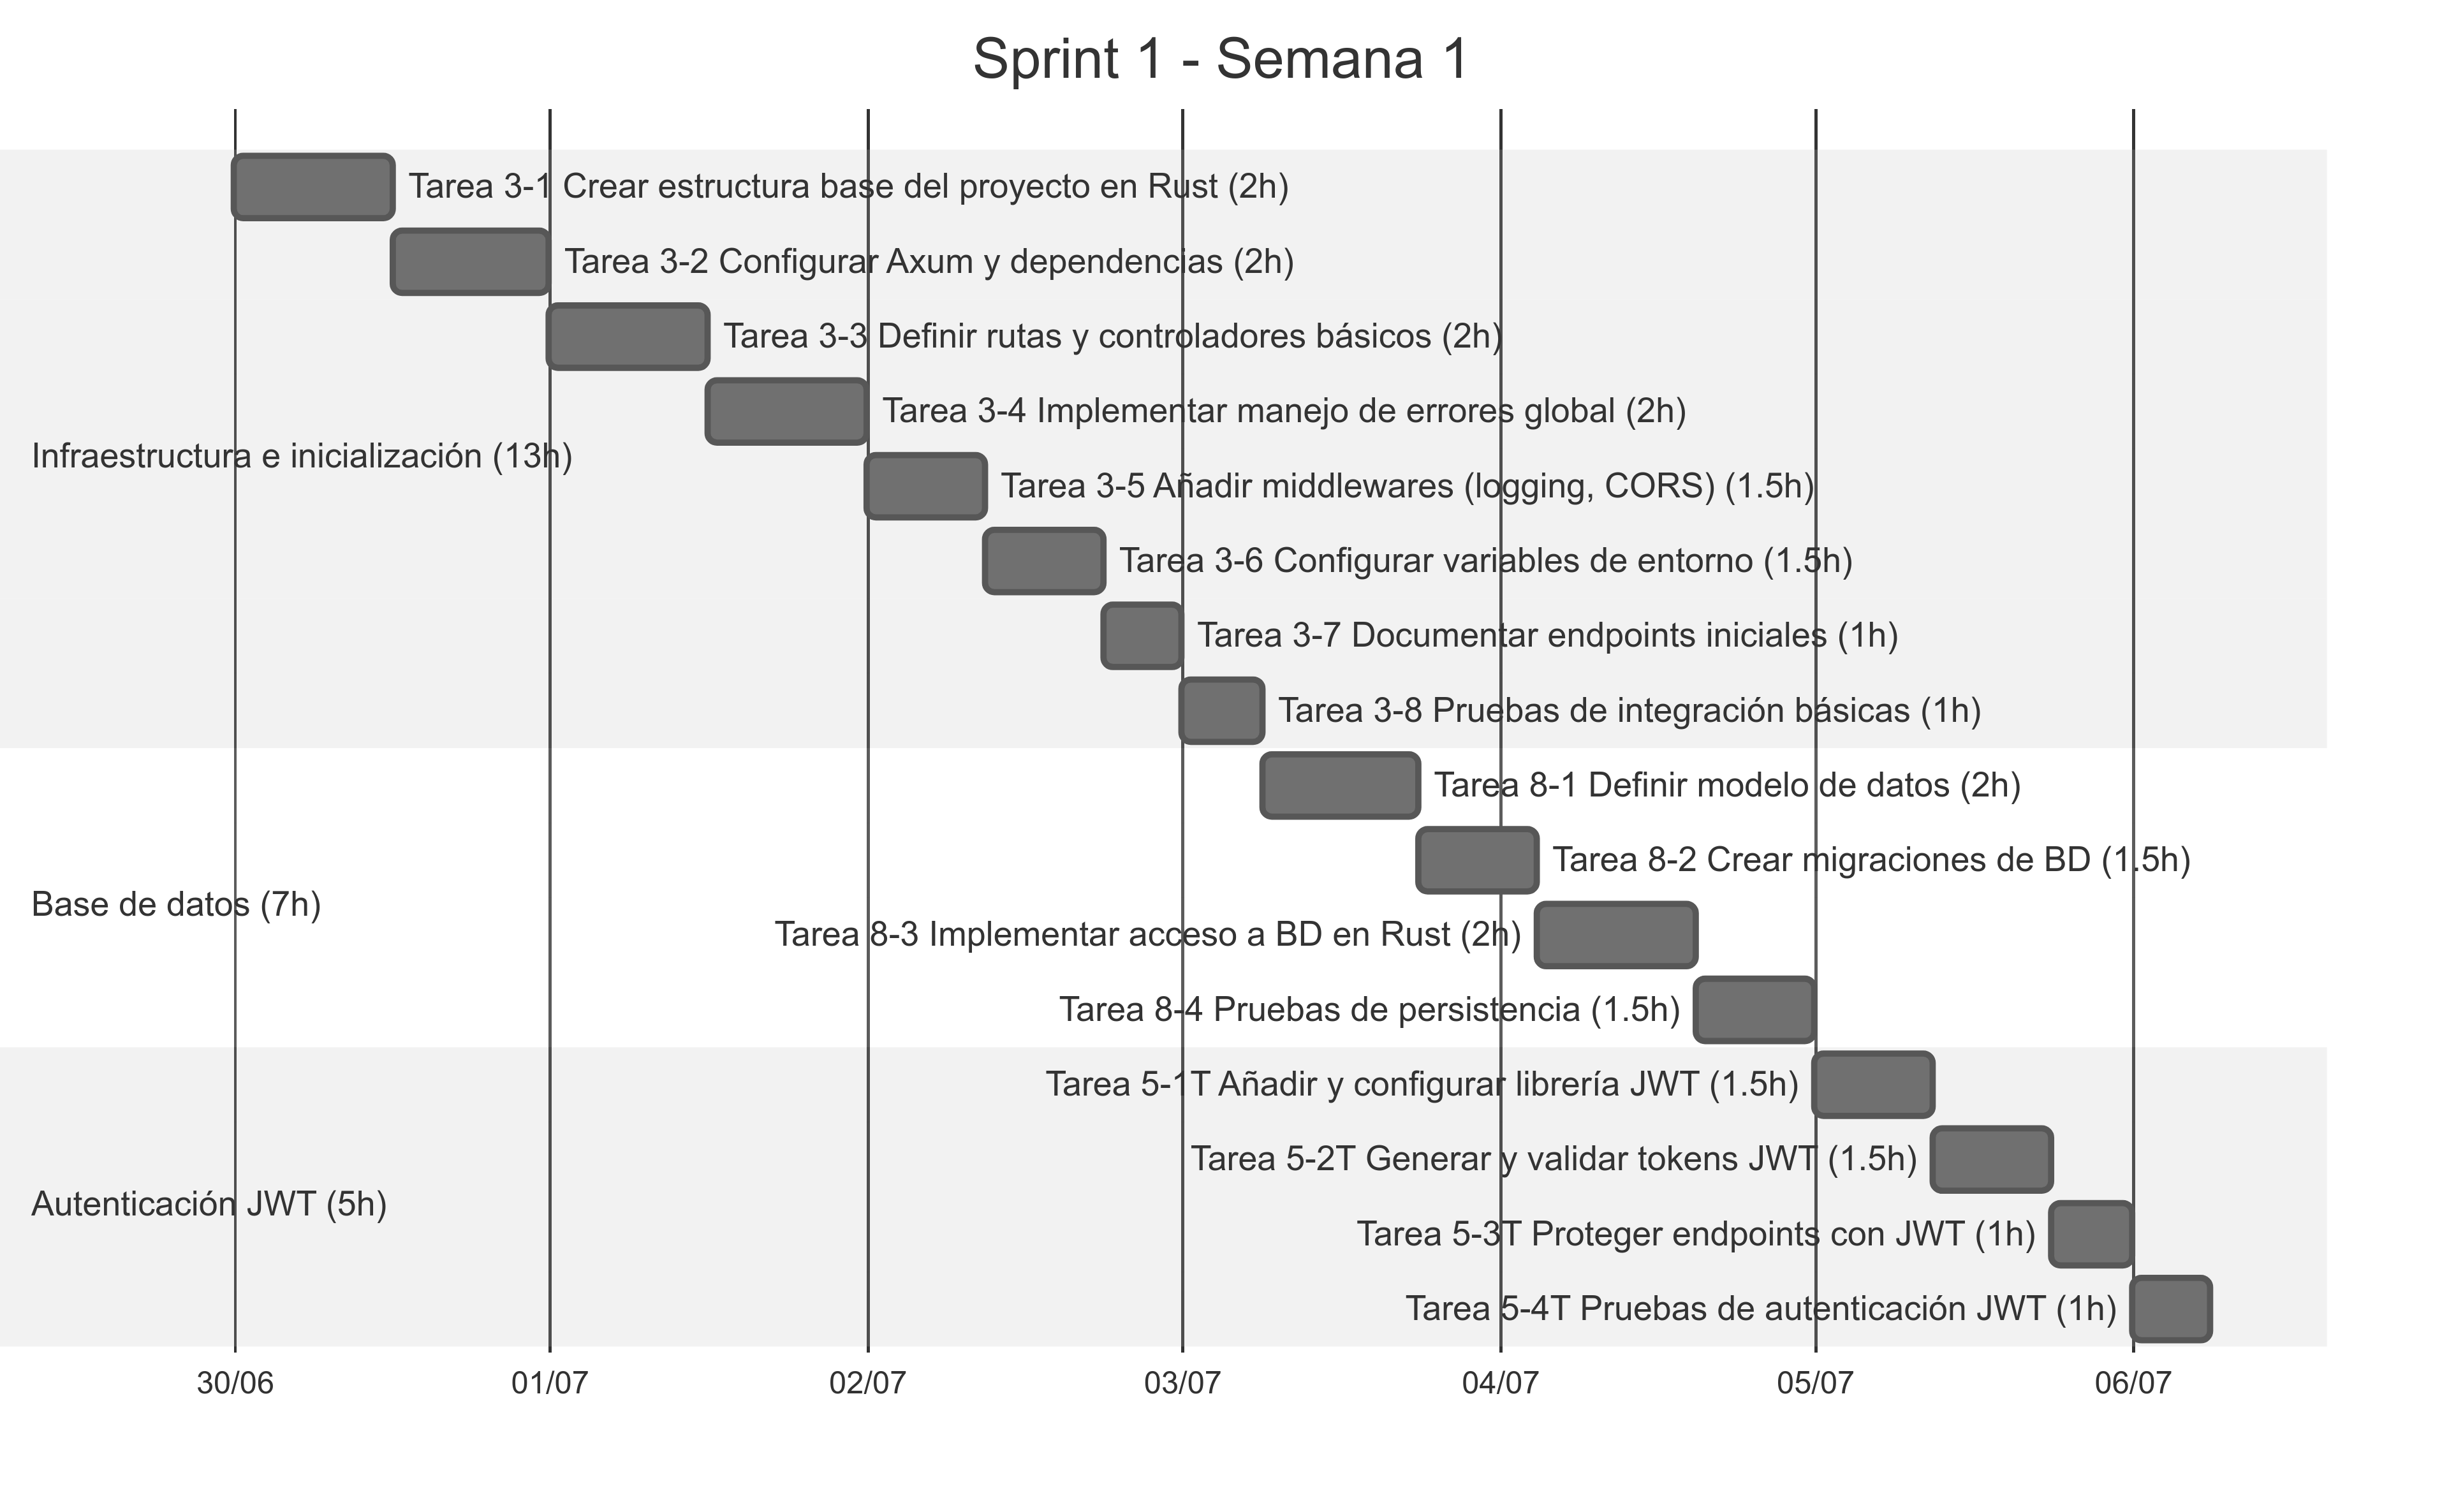
\includegraphics[width=0.8\textwidth]{assets/sprint1/sprint1-week1.png}
    \end{center}
    \caption{Diagrama de Gantt de las tareas de la primera semana del sprint}\label{fig:sprint1-week1}
\end{figure}

\begin{figure}[H]
    \begin{center}
        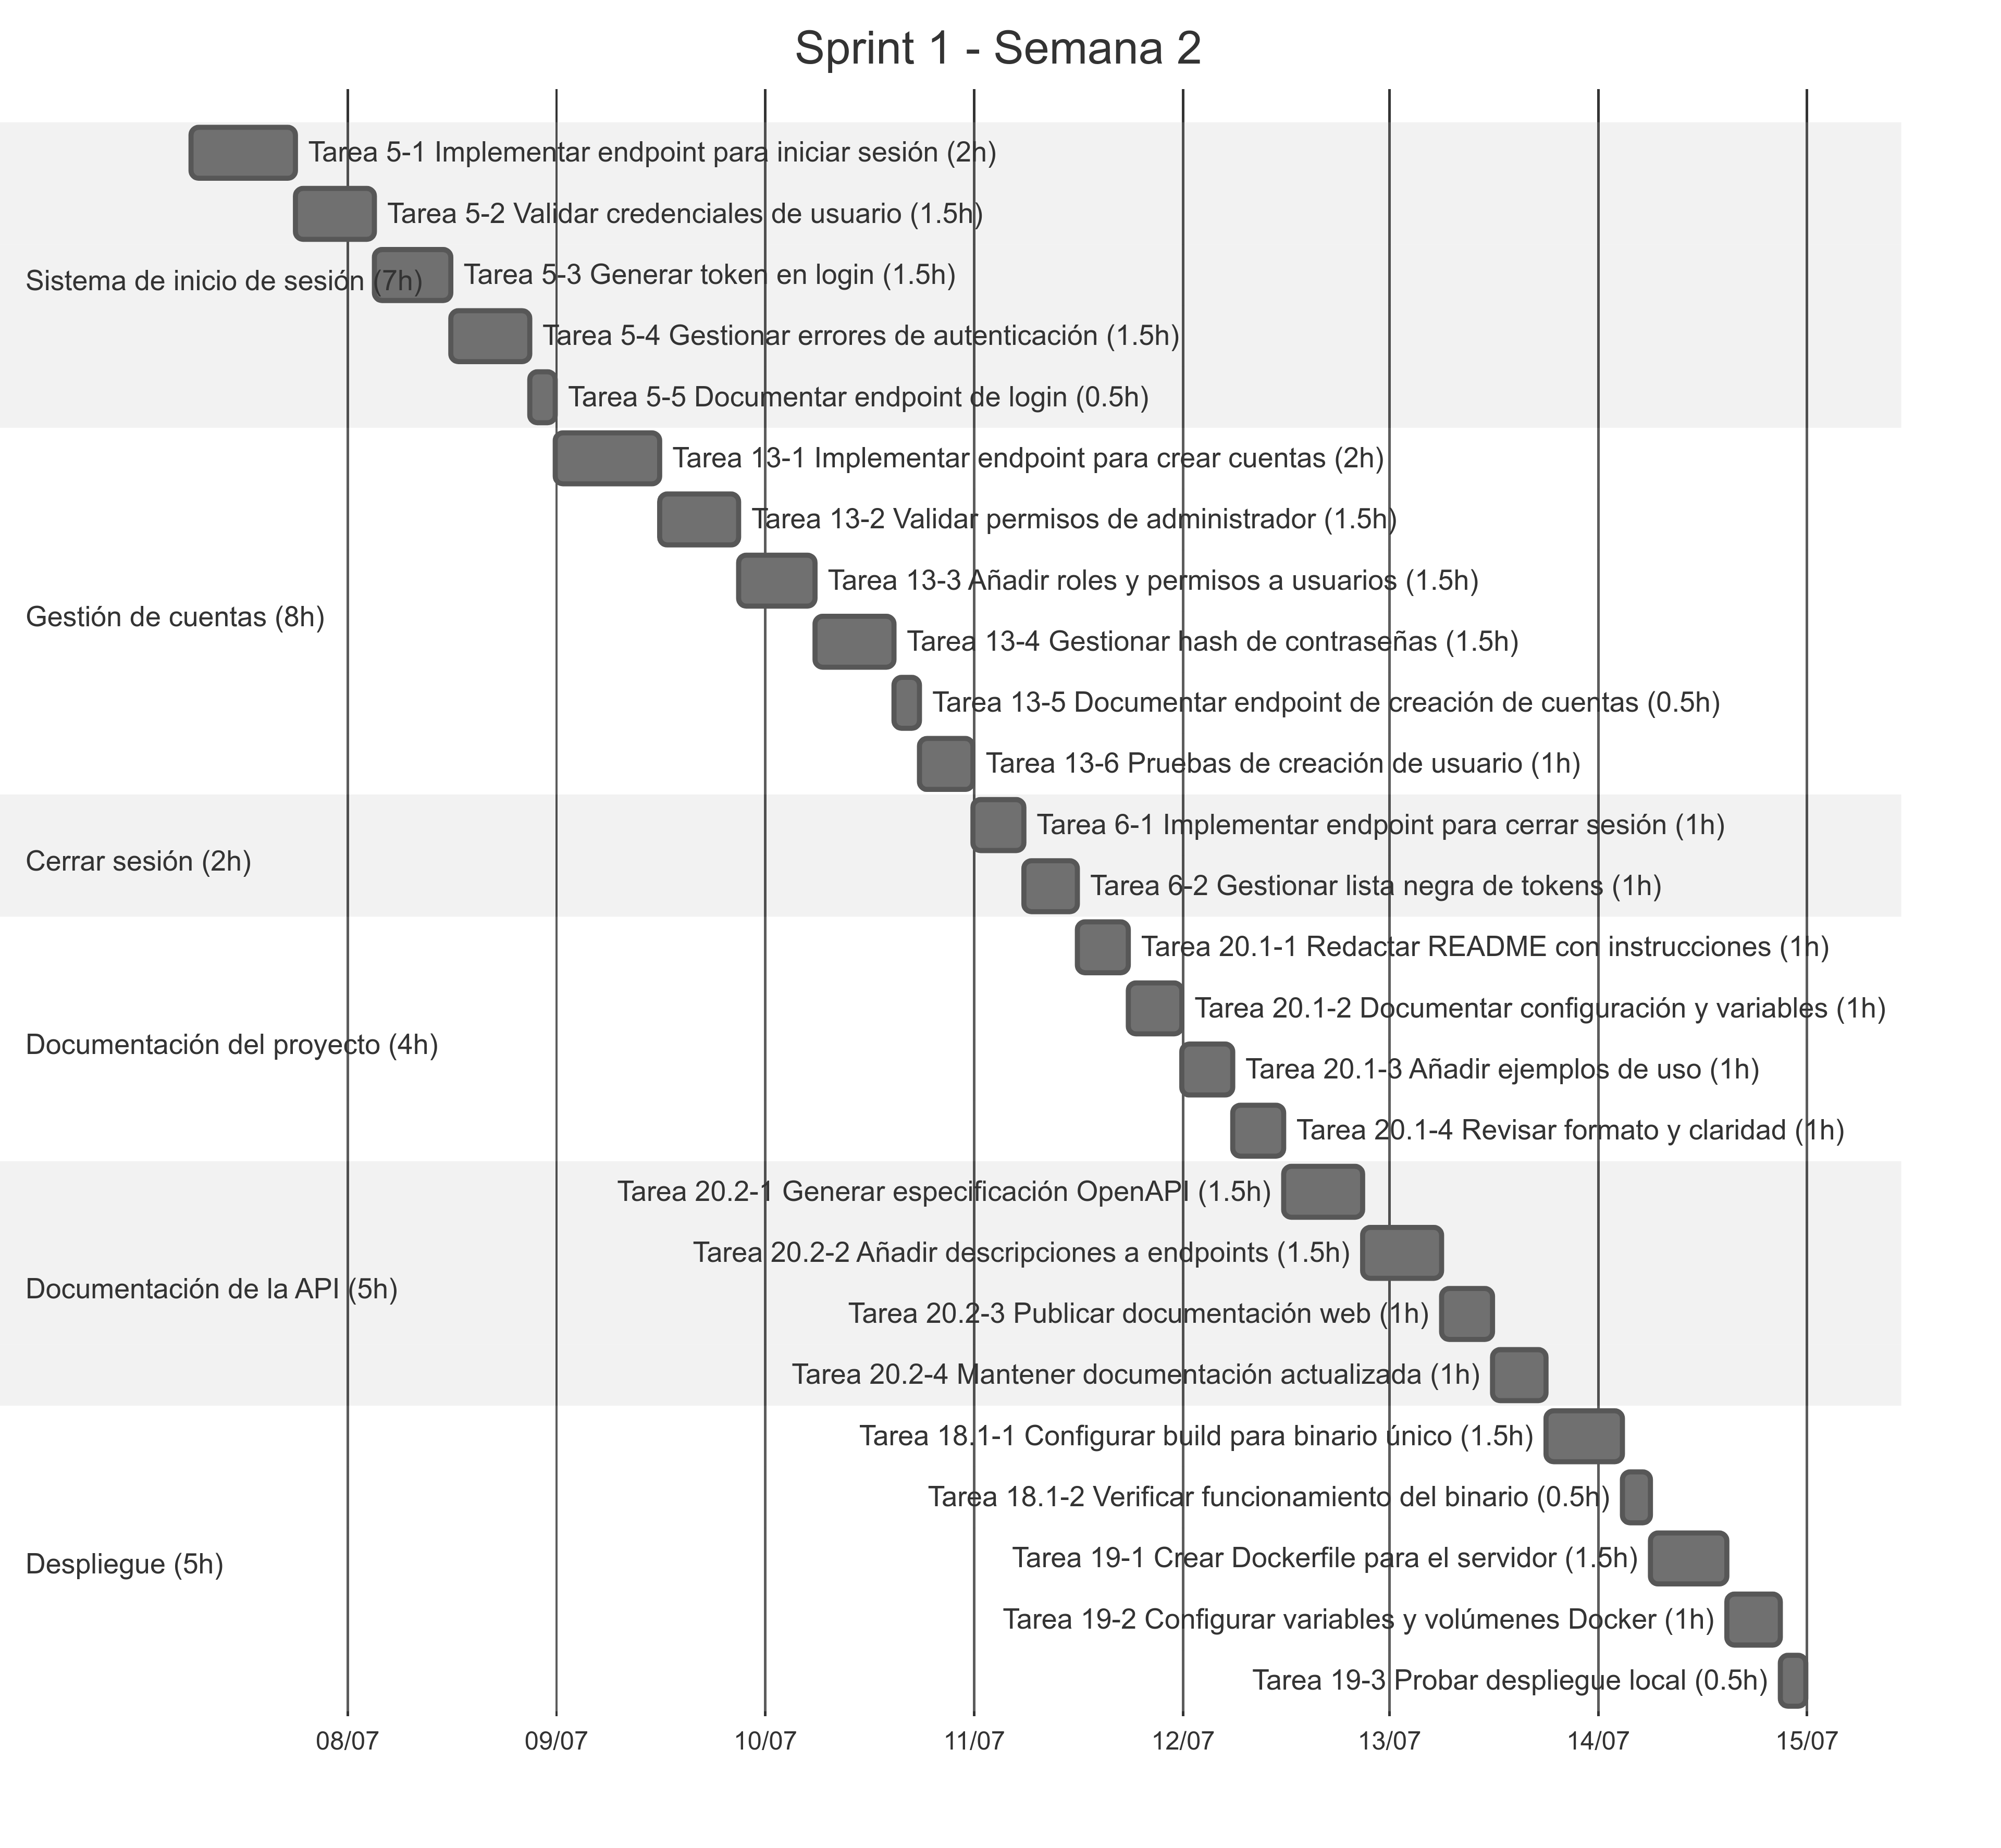
\includegraphics[width=0.8\textwidth]{assets/sprint1/sprint1-week2.png}
    \end{center}
    \caption{Diagrama de Gantt de las tareas de la segunda semana del sprint}\label{fig:sprint1-week2}
\end{figure}

Se ha seguido un orden lógico, en el que primero inicializaremos toda la capa de interfaz, en este caso nuestra API, junto con todas las dependencias que nos harán falta a la hora de documentar, errores no genéricos, variables de entorno, pruebas...

Después, se implementará el diseño de la base de datos. Una vez tenemos esta base, se implementarán las primeras funcionalidades, que van a ser la del inicio de sesión seguro, seguido de la gestión de cuentas. Para finalizar el sprint, se documentará todo al completo.

Para finalizar, configuraremos todo lo necesario para poder desplegar el servidor.

